\chapter{Análise Exploratória do Projeto Mezuro}\label{chap:analise_exploratoria}

O objetivo deste capítulo é registrar os resultados da Análise Exploratória da
plataforma Mezuro. As seções apresentam o contexto em que esta análise foi
realizada, ou seja, quais projetos foram adicionados. Também destaque-se os
resultados obtidos, a comparação com o Code Climate e uma pequena discussão dos
resultados.

Desta forma, é ressaltado a seleção dos projetos do SPB. Dos 71 projetos, 47\% é
desenvolvido em PHP. Quantidade esta que foi decisiva na seleção de quais
softwares seriam avaliados, além de conciliar com o intuito da equipe de
desenvolvimento do SPB de incorporá-lo neste portal.

O resultado dessa análise exploratória é o primeiro conjunto de contribuições
deste trabalho.

\section{Exemplo de Uso: Projetos do Software Público Brasileiro}

O Software Público Brasileiro (SPB) é uma inciativa do Governo Federal que visa
o compartilhamento de softwares, experiências e informações amparado pela tese
do bem público como aquele que apresenta características de indivisibilidade e
de não rivalidade, ou seja, que pode ser usado por todos sem que com isto se
estabeleça competição pelo bem entre os usuários. A disponibilização dos
softwares no SPB é justificada pelo caráter cada vez mais estratégico para
governos e sociedade, pela similaridade de demandas entre os órgãos e entidades
públicas, pela racionalização dos recursos humanos, materiais e de tecnologia
da informação para seu atendimento e pelo acervo de soluções desenvolvidas
pelos diferentes poderes e esferas governamentais \cite{santos2011in01}.

Este capítulo trata da análise das métricas do código-fonte dos projetos do SPB
via Mezuro.

O SPB portanto é uma plataforma \textit{Web} de colaboração integrada. É composto por um
conjunto de ferramentas. São elas \cite{aboutSPB}:

\begin{itemize}
  \item \textbf{Noosfero:} Plataforma \textit{Web} Livre de Redes Sociais, desenvolvida
	em Ruby on Rails. Responsável pelas funcionalidades de gerenciamento de
	conteúdo (CMS) do SPB, permitindo a criação de páginas de usuários, softwares
	e comunidades de forma flexível e customizável. É a ferramenta com maior
	integração com o usuário, pois é responsável pelas páginas dos softwares
	disponibilizados, gerenciamento dos downloads destes softwares, criação de
	notícias e categorização dos softwares;
  \item \textbf{Mailman:} É uma aplicação para gerenciamento de listas de
	e-mail, escrito majoritariamente em Python e faz parte do projeto GNU. Cada
	software disponibilizado no SPB possui sua própria lista de e-mail e ela é um
	dos meios de comunicação entre os administradores e usuários dos softwares.
	Também serve para divulgação de notícias ou relatórios de novas versões.
	Possibilita ao usuário a participação em tópicos de discussão respondendo
	através do próprio e-mail, sem a necessidade de acessar diretamente o SPB;
	\item \textbf{Gitlab:} Gerenciador de repositórios Git com funcionalidades de
	\textit{wiki} e mapeamento de \textit{issues}, escrito em Ruby;
	\item \textbf{Mezuro:} Plataforma \textit{Web} Livre para avaliação colaborativa de
	código fonte, desenvolvido em Ruby on Rails, também adicionada ao SPB para
	fornecer acompanhamento da qualidade do código dos projetos \cite{aboutSPB}.
\end{itemize}

A integração das ferramentas acima citadas é realizada por meio do
\textbf{Colab}, um software desenvolvido em Python e Django que suporta
ambientes colaborativos e agregados. Em resumo, é uma plataforma para
autenticação, buscas e inserção de conteúdo no SPB \cite{aboutSPB}.

\begin{figure}[!htb]
	\centering
    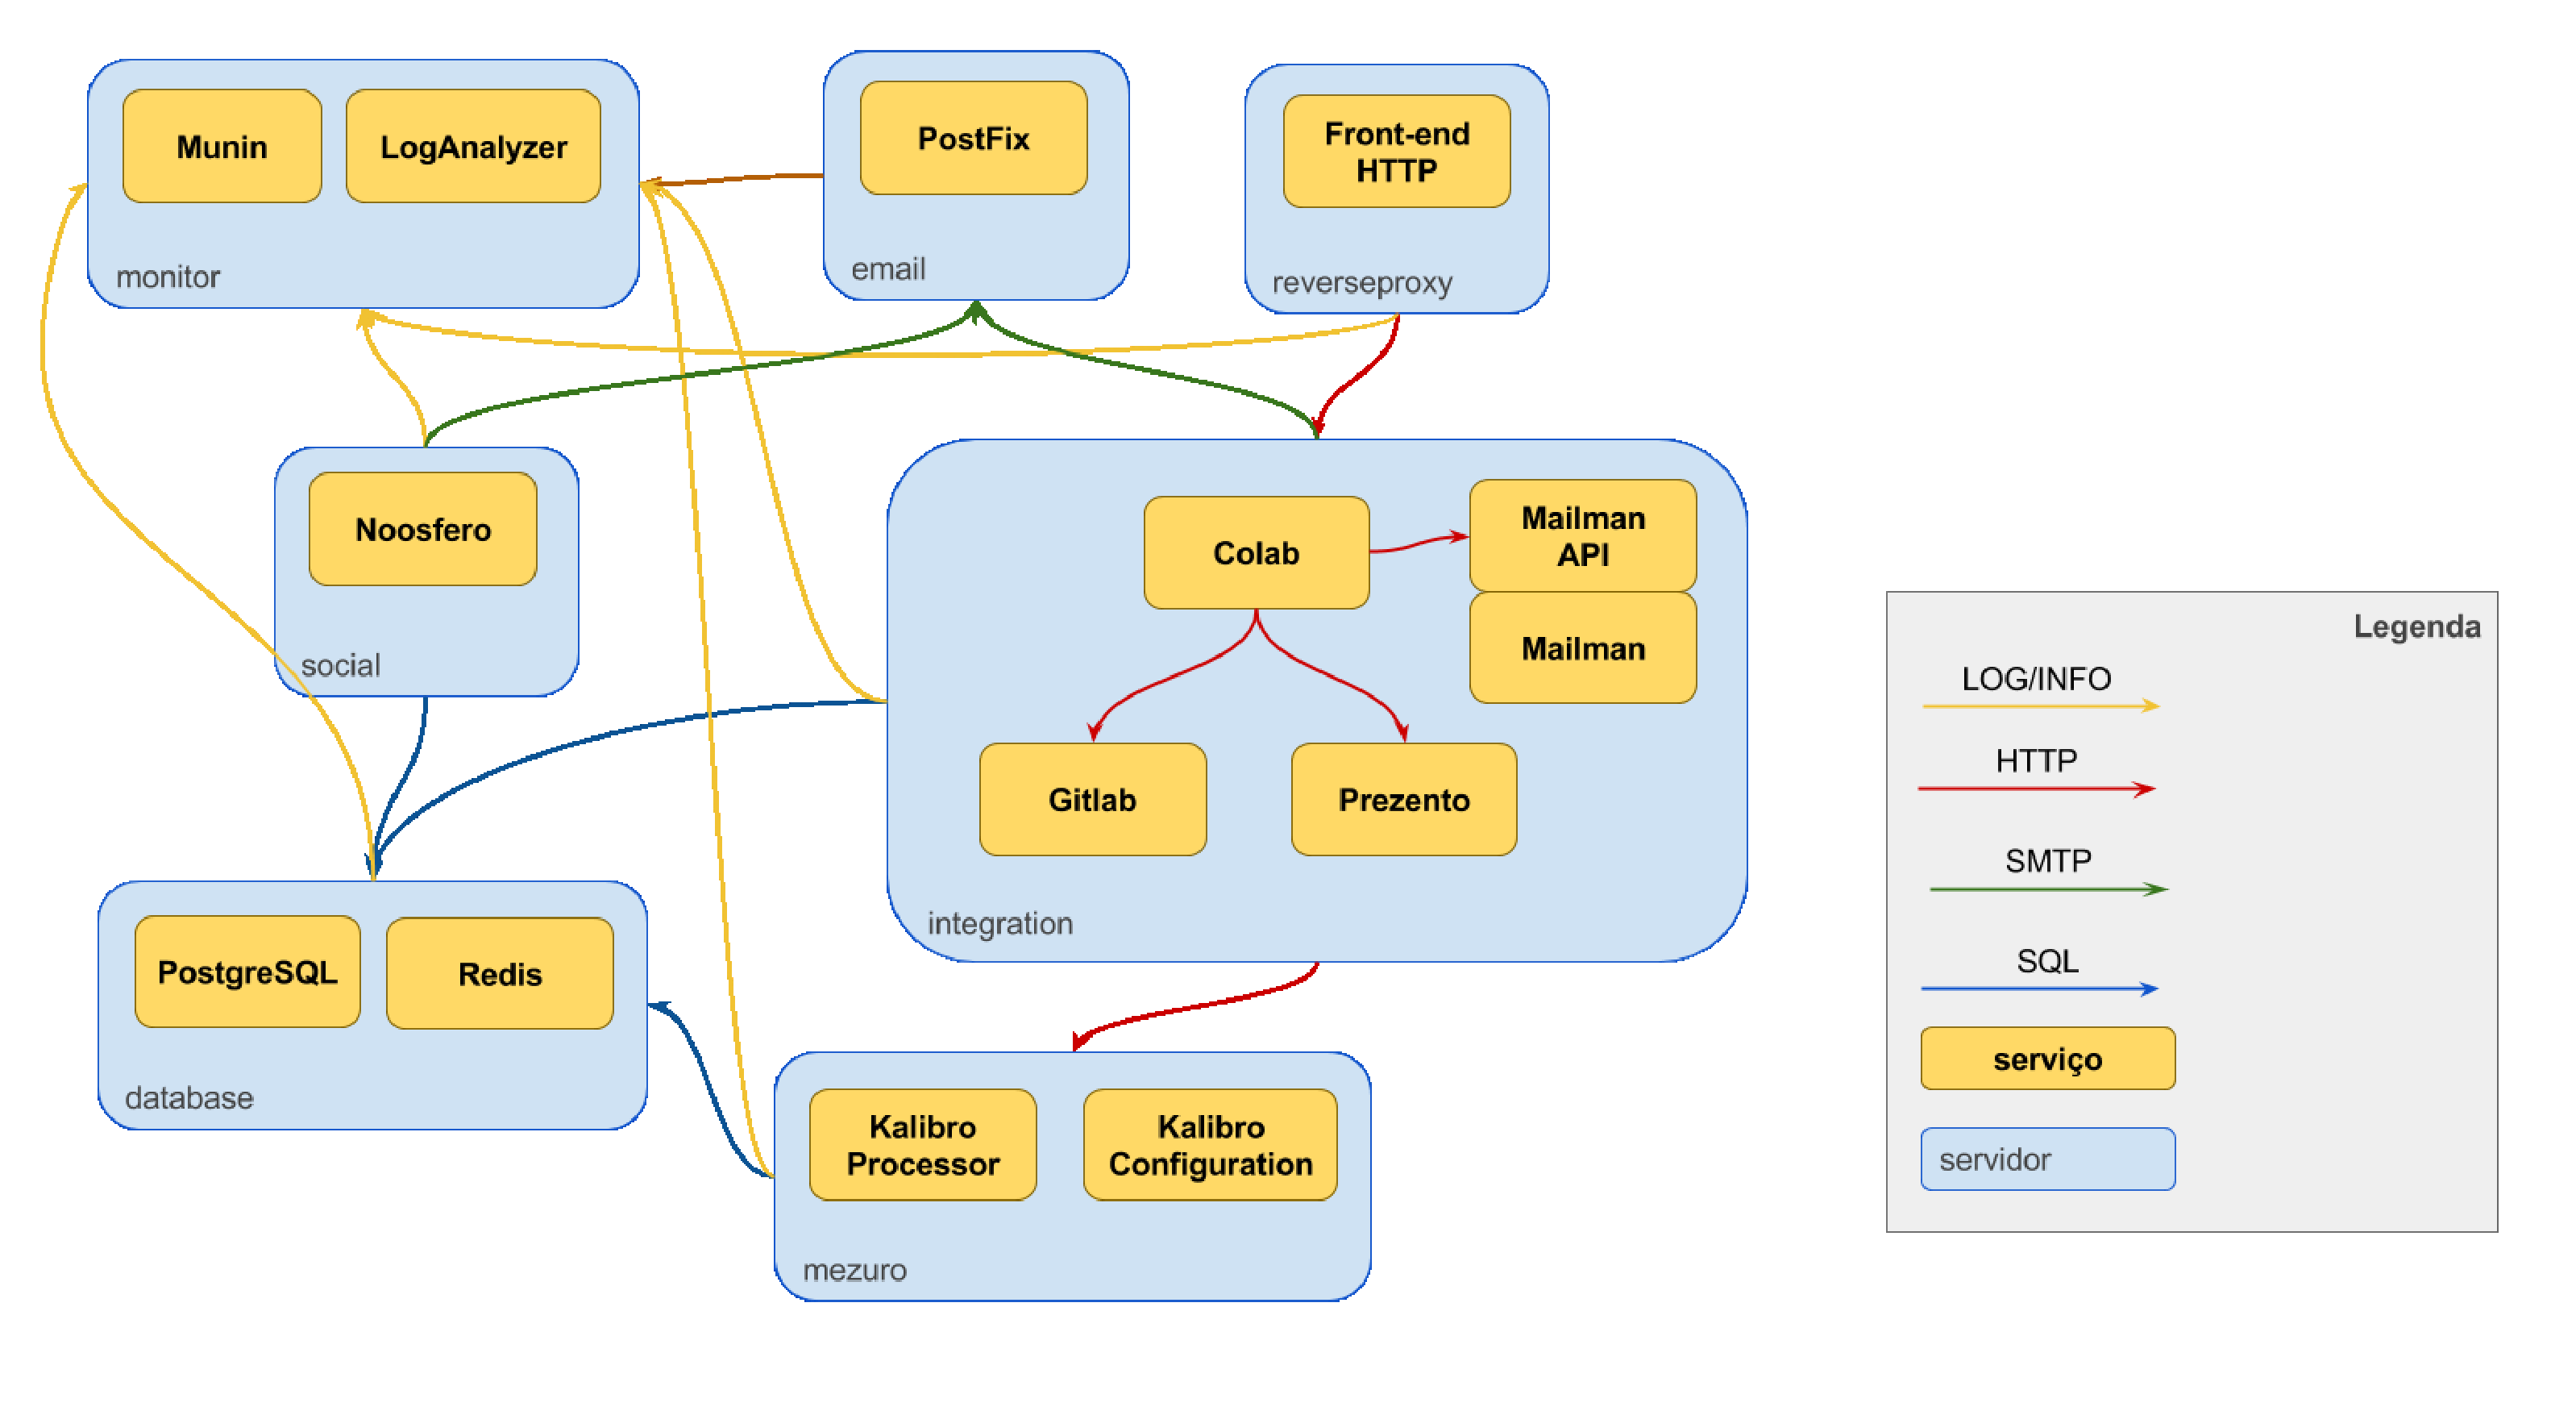
\includegraphics[keepaspectratio=true,scale=0.3]
    {figuras/arquitetura_spb.eps}
  \caption{Representação da Arquitetura do SPB}
  \label{fig:arquitetura_spb}
\end{figure}

Do ponto de vista arquitetural, são necessárias 7 máquinas/servidores para
executar atualmente o Portal do
Software Público Brasileiro. Cada máquina representa uma função distinta. O
acesso \textit{SSH} à essas máquinas é limitado à configurações de ordem de
prioridade e portas específicas. Os detalhes podem ser verificados na
referência \cite{archSPB}. As sete máquinas são:

\begin{itemize}
  \item \textbf{Reverseproxy:}
  \begin{itemize}
    \item Proxy Reverso
  \end{itemize}

  \item \textbf{Integration:}
    \begin{itemize}
      \item Segundo Proxy Reverso
      \item Repositórios Git
      \item Listas de e-mail
      \item Back-End final de e-mail
    \end{itemize}

  \item \textbf{E-mail}
  \begin{itemize}
    \item Relay de e-mail
  \end{itemize}

  \item textbf{Social}
  \begin{itemize}
    \item Servidor da Rede Social Noosfero
  \end{itemize}

  \item \textbf{Database}
  \begin{itemize}
    \item{Servidor de Banco de Dados PostgreSQL}
  \end{itemize}

  \item \textbf{Mezuro}
  \begin{itemize}
    \item Servidor dedicado para análise de código com o Mezuro
  \end{itemize}

  \item \textbf{Monitor}
  \begin{itemize}
    \item Monitoramento de informações dos outros serviços
  \end{itemize}
\end{itemize}

\subsection{Categorização dos Projetos do SPB}

Foi realizado uma categorização dos softwares disponibilizados no Portal do
Software Público Brasileiro, como insumo que corroborará com as hipóteses
levantadas neste trabalho. A adição dos softwares do SPB à ferramentas de
monitoramento (Mezuro e Code Climate\footnote{\url{https://codeclimate.com/}})
foi planejada para que o código seja avaliado e para que haja um incentivo aos
desenvolvedores e administradores das comunidades do Portal ao monitoramento de
seus projetos. Esta adição ou contribuição foi registrada e está disponível
para acesso por meio deste trabalho ou na lista de discussão para
desenvolvedores do SPB.

Como explicado na seção anterior, uma das ferramentas do SPB é o Gitlab
(serviço para armazenamento de repositórios Git) e foi constatado que
aproximadamente 75\% dos softwares \textbf{não} possuem seus códigos-fonte
versionados nesta ferramenta. Realizado algumas pesquisas, foi encontrado o
código-fonte em outros serviços (Github, Bitbucket). Fato esse que já auxiliou
neste primeiro desafio de adicionar determinados softwares para avaliação no
Mezuro. Porém, se considerarmos o SPB como a plataforma de colaboração
integrada, colaboração que é um dos objetivos fundamentais ao Governo Federal
com o Portal, o infortúnio de ter aproximadamente três-quartos dos softwares
não versionados é algo que atinge toda a comunidade que utiliza o SPB: sejam
desenvolvedores interessados em contribuir/evoluir os softwares; sejam usuários
finais que também contribuem com registro de problemas, ou issues, ou \textit{bugs}.

Por padrão, no momento da disponibilização de um novo software no SPB, já são
criadas ``instâncias'' de cada uma das ferramentas que compõem o Portal. Bastando
ao administrador adequar o código-fonte ao versionamento com o Git. Por exemplo
o software ``xpto'', teria o seguinte domínio para acesso ao código fonte:
softwarepublico.gov.br/gitlab/xpto/xpto.

Como solução, durante a categorização, foi realizado o ``commit inicial'' para
aqueles softwares que disponibilizaram o código-fonte por meio de arquivo
compactado. Como forma de centralização e organização, foi criado a organização
``spb-metrics'' no Github\footnote{\url{https://github.com/spb-metrics}}, pois
para avaliação no Code Climate, os repositórios precisam estar neste serviço e
serem públicos. De outra maneira, ou em outro serviço, a avaliação teria um
custo estipulado pelas regras de negócio do próprio Code Climate. Já no Mezuro é
possível adicionar um repositório para avaliação independentemente do serviço
(Github, Gitlab, Bitbucket, etc), basta ser utilizado o sistema de controle de
versão Git ou SVN. Comparação esta que reforça o estudo da visualização de
software como possível auxílio e contribuição ao Mezuro. A categorização
completa dos softwares do SPB está no final da próxima seção deste capítulo.

\begin{figure}[!htb]
	\centering
    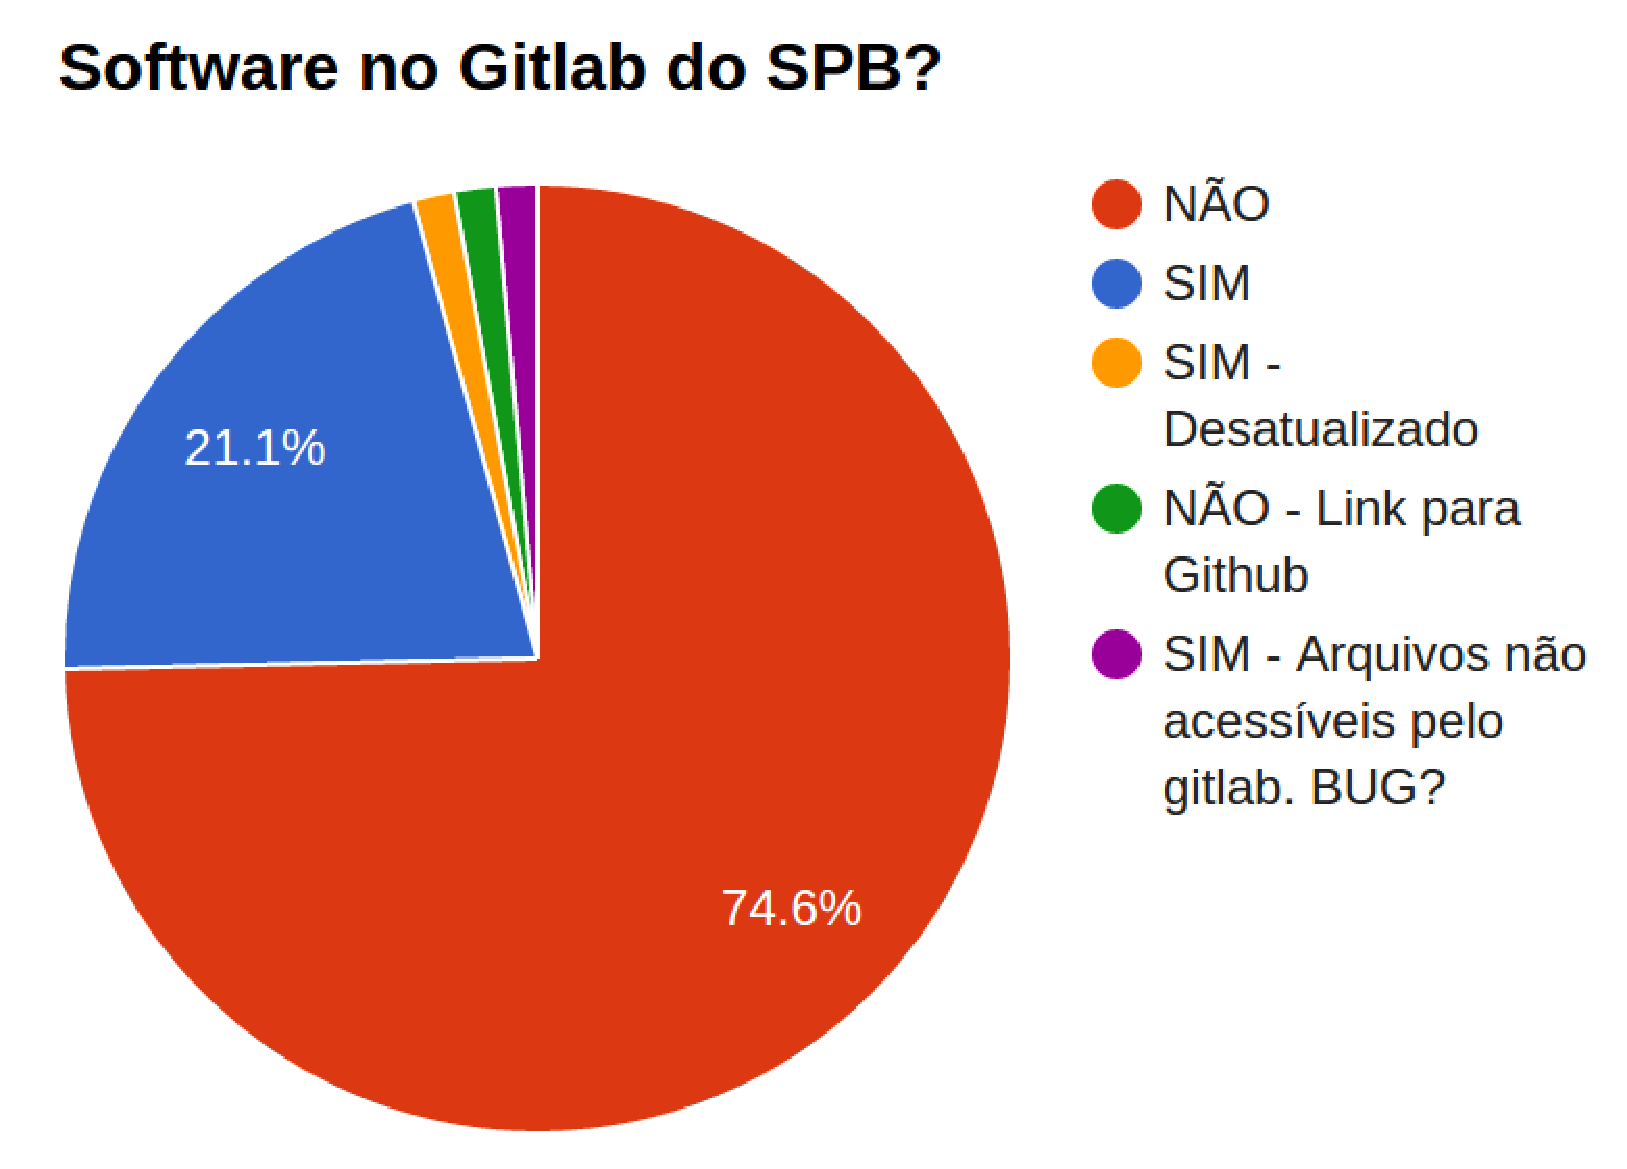
\includegraphics[keepaspectratio=true,scale=0.45]
    {figuras/is_software_gitlab_spb.eps}
  \caption{Porcentagem de Softwares Versionados no Gitlab do SPB}
  \label{fig:is_software_gitlab_spb}
\end{figure}

\begin{figure}[!htb]
	\centering
    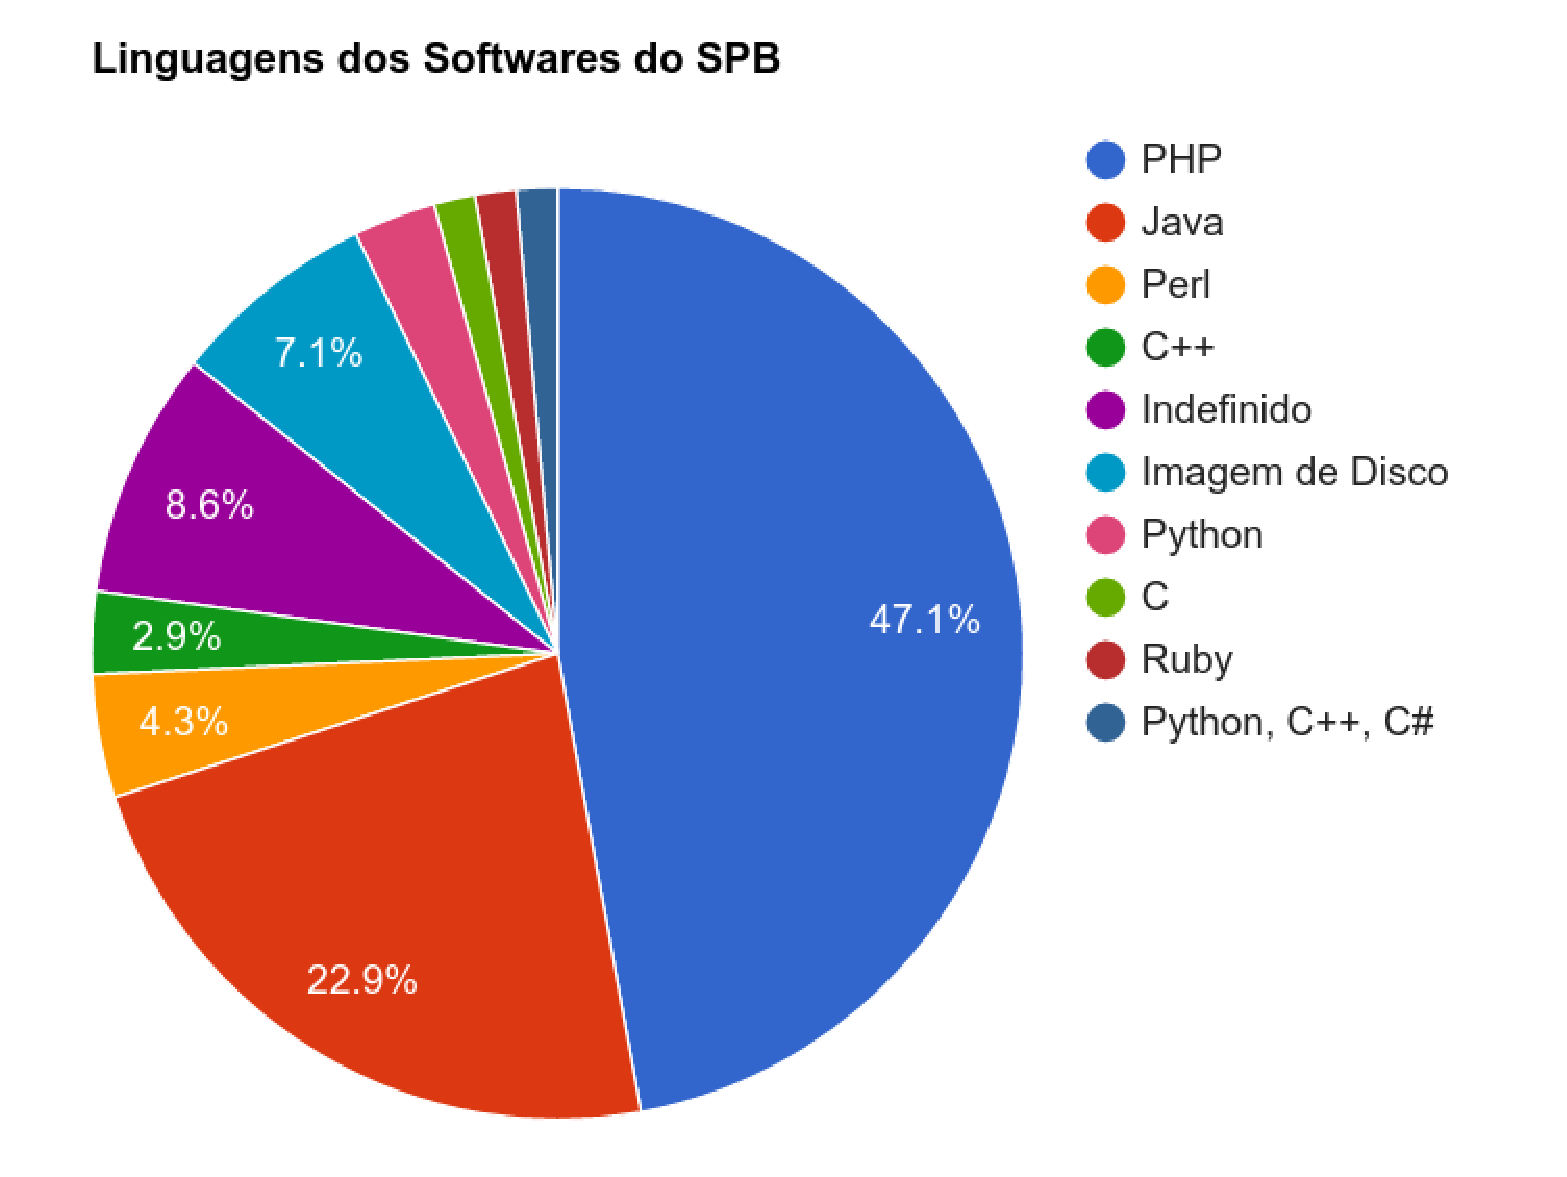
\includegraphics[keepaspectratio=true,scale=0.5]
    {figuras/linguagens_softwares_spb_v2.eps}
  \caption{Linguagens em que os Softwares do SPB são desenvolvidos}
  \label{fig:linguagens_softwares_spb_v2}
\end{figure}

\newpage

As Figuras \ref{fig:is_software_gitlab_spb} e \ref{fig:linguagens_softwares_spb_v2}
mostram respectivamente o percentual de softwares com repositório Git no SPB e
em qual linguagem foram escritos predominantemente. Com 47\%, PHP é a linguagem
em que é desenvolvido a maioria dos softwares do Portal SPB. Seguido por Java,
com 23\% e outras (Python, C++, Perl), sendo menos de 5\% cada. Foi decidido
portanto iniciar a avaliação de softwares escritos em PHP e com código-fonte
disponibilizado (compactado ou versionado).

\newpage

\section{O uso do Mezuro e do Code Climate}

O Code Climate é uma plataforma aberta e extensível de análise estática de código
que ajuda desenvolvedores a manter o seu software com determinado nível de
qualidade. Esta análise é feita a cada novo \textit{commit},
\textit{pull request} ou \textit{branch}. A vinculação da conta é feita através
do Github e a avaliação do código é gratuita enquanto o repositório estiver em
uma conta no Github e for público necessariamente. Esta gratuidade é até um dos
slogans da ferramenta: \textit{Code Climate is 100\% free for Open Source,
forever. Add your Open Source GitHub repo.} (O Code Climate é 100\% grátis para
projetos de código aberto, para sempre. Adicione o seu repositório público do
Github.) Para repositórios privados ou de outros sistemas de hospedagem remota de
código (Gitlab, Bitbucket), é cobrado uma taxa de 25 dólares até a data de
escrita deste trabalho. Porém, uma alternativa para projetos privados é utilizar
a interface de linha de comandos com o comando do próprio Code Climate (Code
Climate - CLI\footnote{https://github.com/codeclimate/codeclimate}) e executar a
análise localmente ou em um container Docker \cite{codeClimateDoc}.

Atualmente, o Code Climate faz a análise dos códigos nas seguintes linguagens:
CSS, Go, Javascript, PHP, Python e Ruby. E também para as seguintes ferramentas,
tecnologias, linguagens ou \textit{frameworks}: Apex, CoffeScript, Ember, ESLint,
Haskell, Haxe, RubyMotion, Rails, SCSS, Swift e Vim Script \cite{codeClimateDoc}.
Em comparação com o Mezuro, a análise de C, C++ e Java é um diferencial, graças
ao Analizo, como citado no Capítulo \ref{chap:mezuro}.

\begin{figure}[!htb]
	\centering
    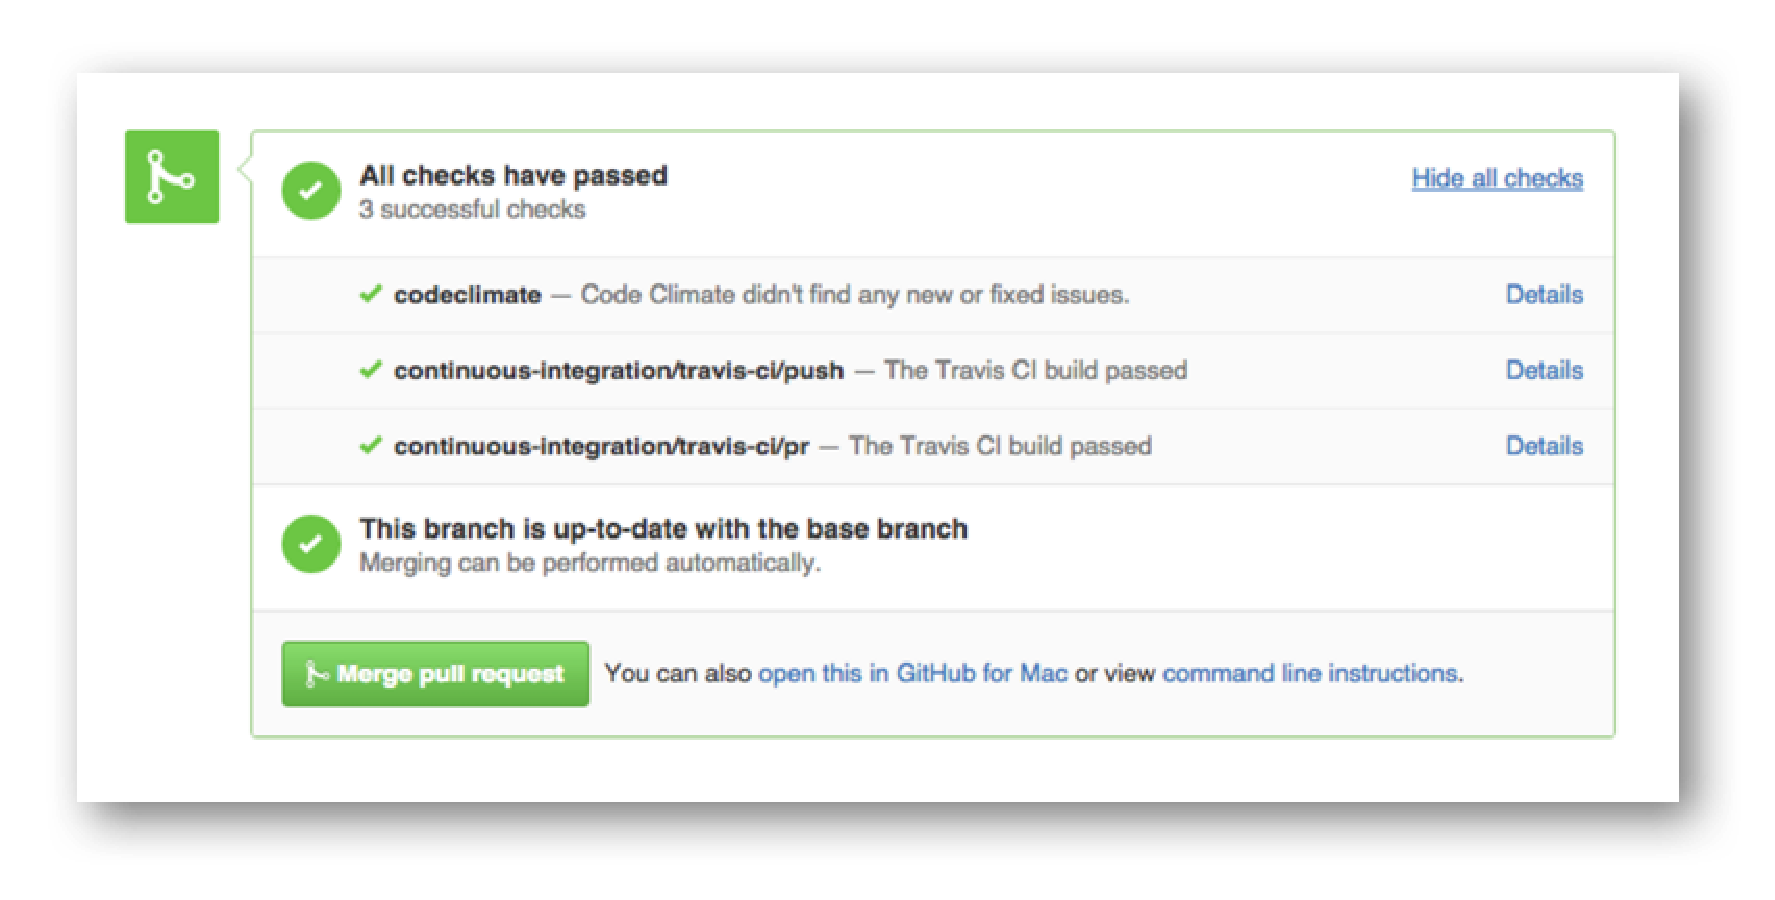
\includegraphics[keepaspectratio=true,scale=0.5]
    {figuras/github_workflow_with_codeclimate.eps}
  \caption{Fluxo de submissão do Github com o Code Climate incorporado}
  \label{fig:github_workflow_with_codeclimate}
\end{figure}

\begin{figure}[!htb]
	\centering
    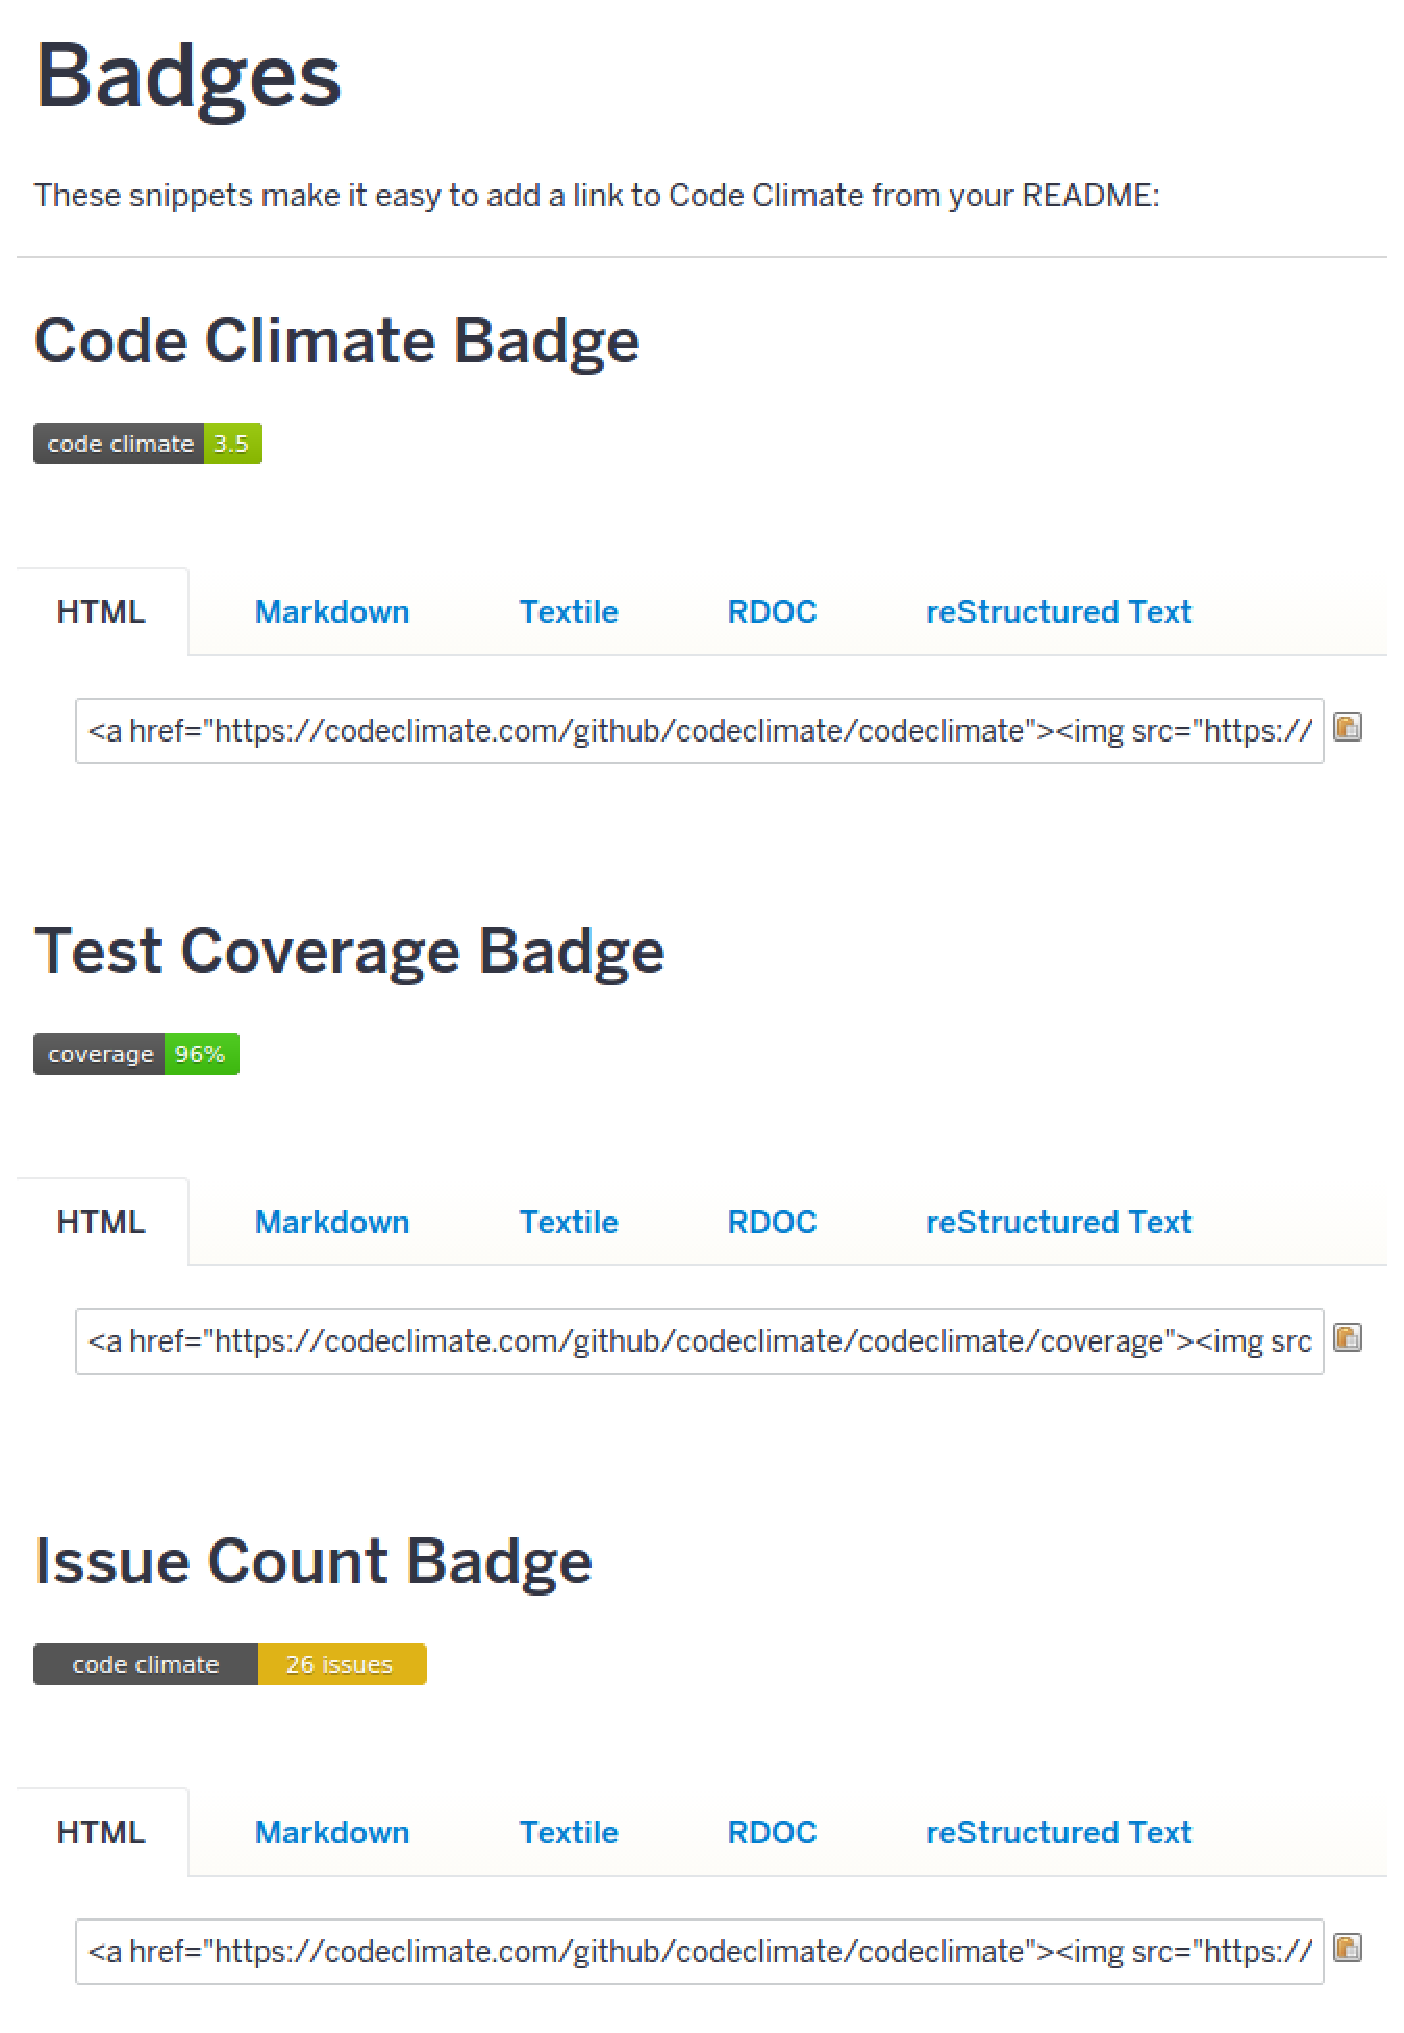
\includegraphics[keepaspectratio=true,scale=0.5]
    {figuras/codeclimate_badges.eps}
  \caption{Insígnias/Emblemas do Code Climate}
  \label{fig:codeclimate_badges}
\end{figure}

\newpage

Alguns dos diferenciais do Code Climate são: exposição de trechos de códigos que
apresentam possíveis problemas e/ou necessitam de refatoração; a incorporação da
análise prévia de um \textit{pull request} no fluxo de submissão do Github (vide
Figura \ref{fig:github_workflow_with_codeclimate}); e a
atribuição de \textit{badges} (insígnias, emblemas) para ser utilizado em uma
página \textit{Web} ou no \textit{README} do Github, disponíveis em seis
linguagens de marcação (HTML, Markdown, Textile, RDOC, reStructured Text).
Esses \textit{badges} (Figura \ref{fig:codeclimate_badges}) podem ser utilizados
para expor a nota do projeto, a porcentagem de cobertura de teste e a contagem
de \textit{issues} identificadas pelo Code Climate \cite{codeClimateDoc}. A
equipe do Mezuro em 2013 mapeou a possibilidade de incorporação de \textit{badges}
na plataforma. Porém, pouco se discutiu sobre o assunto e a demanda continua em
aberto\footnote{\url{https://github.com/mezuro/prezento/issues/11}}.

Um ponto em semelhança com o Mezuro é a utilização do mesmo \textit{engine}
geral para a linguagem PHP: o PHPMD. A análise de projetos em PHP no Code Climate
é a junção da avaliação dos seguintes motores de análises \cite{codeClimateDoc}:

\begin{itemize}
  \item \textbf{CSSLint:} como esperado de uma ferramenta \textit{lint}, esse
	motor faz uma análise estática do código CSS e aponta padrões que podem ser
	erros ou que possivelmente podem causar problemas aos desenvolvedores;
	\item \textbf{Duplication:} este motor analisa e indica estruturas ou blocos
	de códigos semelhantes;
	\item \textbf{ESLint:} outra ferramenta \textit{lint}, porém para análise e
	verificação de estilo de códigos escritos em EcmaScript ou Javascript;
	\item \textbf{FIXME:} realiza uma busca sensível à caixa alta por palavras
	como \textbf{TODO, FIXME, HACK, BUG} e destaca essas informações reforçando a
	importância ao desenvolvedor, que provavelmente deve consertar alguma parte no
	código agora, não depois;
	\item \textbf{PHP Code Sniffer:} análise estática no código PHP que detecta
	violações de um padrão já definido e estabelecido pela comunidade;
	\item \textbf{PHP Mess Detector:} procura por diferentes potenciais problemas
	com o código escrito em PHP, como possíveis \textit{bugs}, código desnecessário,
	expressões demasiadamente complicadas, e parâmetros ou métodos não utilizados.
\end{itemize}

\begin{figure}[h]
  \centering
    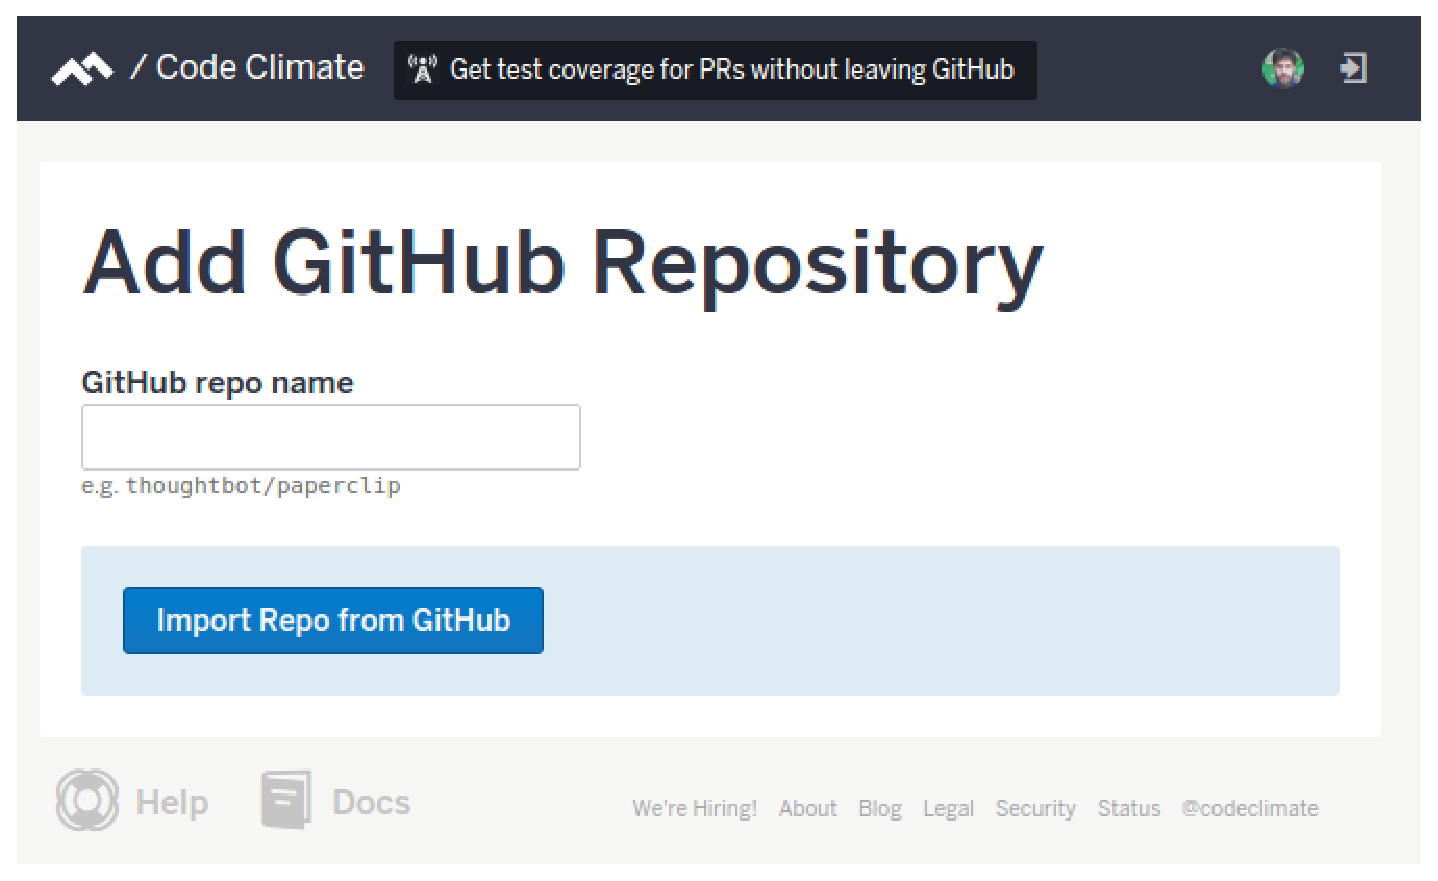
\includegraphics[keepaspectratio=true,scale=0.48]
    {figuras/form_codeClimate.eps}
  \caption{Code Climate - Formulário de adição de repositório para análise}
  \label{fig:form_codeClimate}
\end{figure}

\newpage

A Figura \ref{fig:form_codeClimate} mostra o formulário para a importação de um
repositório e análise no Code Climate. Basta informar o nome do repositório; a
própria ferramenta identifica qual a linguagem predominante e organiza as
\textit{engines} necessárias para a coleta e análise das métricas.

\begin{figure}[!htb]
	\centering
    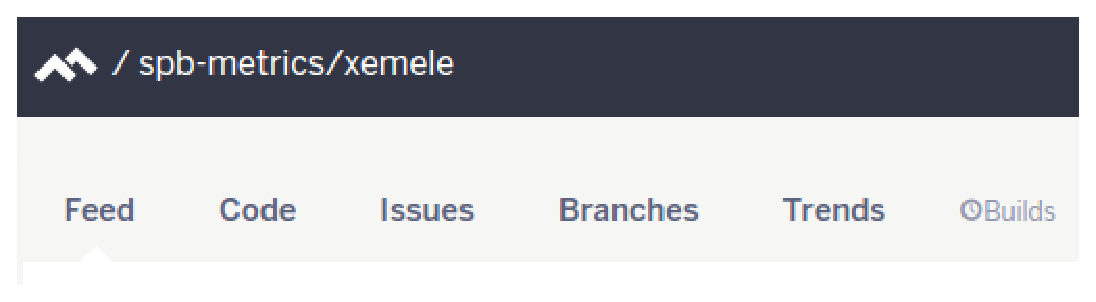
\includegraphics[keepaspectratio=true,scale=0.5]
    {figuras/codeclimate_abas.eps}
  \caption{Code Climate - Abas da Página dos Resultados da Análise}
	\label{fig:codeclimate_abas}
\end{figure}

No Code Climate, o resultado é exposto em uma página com as abas representadas
na Figura \ref{fig:codeclimate_abas}. Cada uma com determinado propósito:
\textit{Feed}, para mostrar um resumo das análises a cada \textit{commit}; a aba
\textit{Code} mostra a nota de cada um dos arquivos, o número de linhas (\textit{LOC}),
a quantidade de vezes que ele foi modificado (\textit{Churn}) e a quantidade de
\textit{issues} relacionadas com aquele arquivo; a aba \textit{Issues} lista as
métricas coletadas com os trechos dos códigos onde foram atribuídos os problemas,
podendo ser filtrado por categoria e \textit{engine}; na aba \textit{Branches},
é exposto a lista de ramos de desenvolvimento do projeto, onde o usuário pode
comparar cada um com o ramo principal; a aba \textit{Trends} mostra por meio de
gráficos, a evolução da nota e da qualidade do código; e finalmente, na aba
\textit{Builds} há a exibição da lista das vezes que o projeto foi ``construído''
para a análise, com sucesso ou não.

\begin{figure}[!htb]
	\centering
    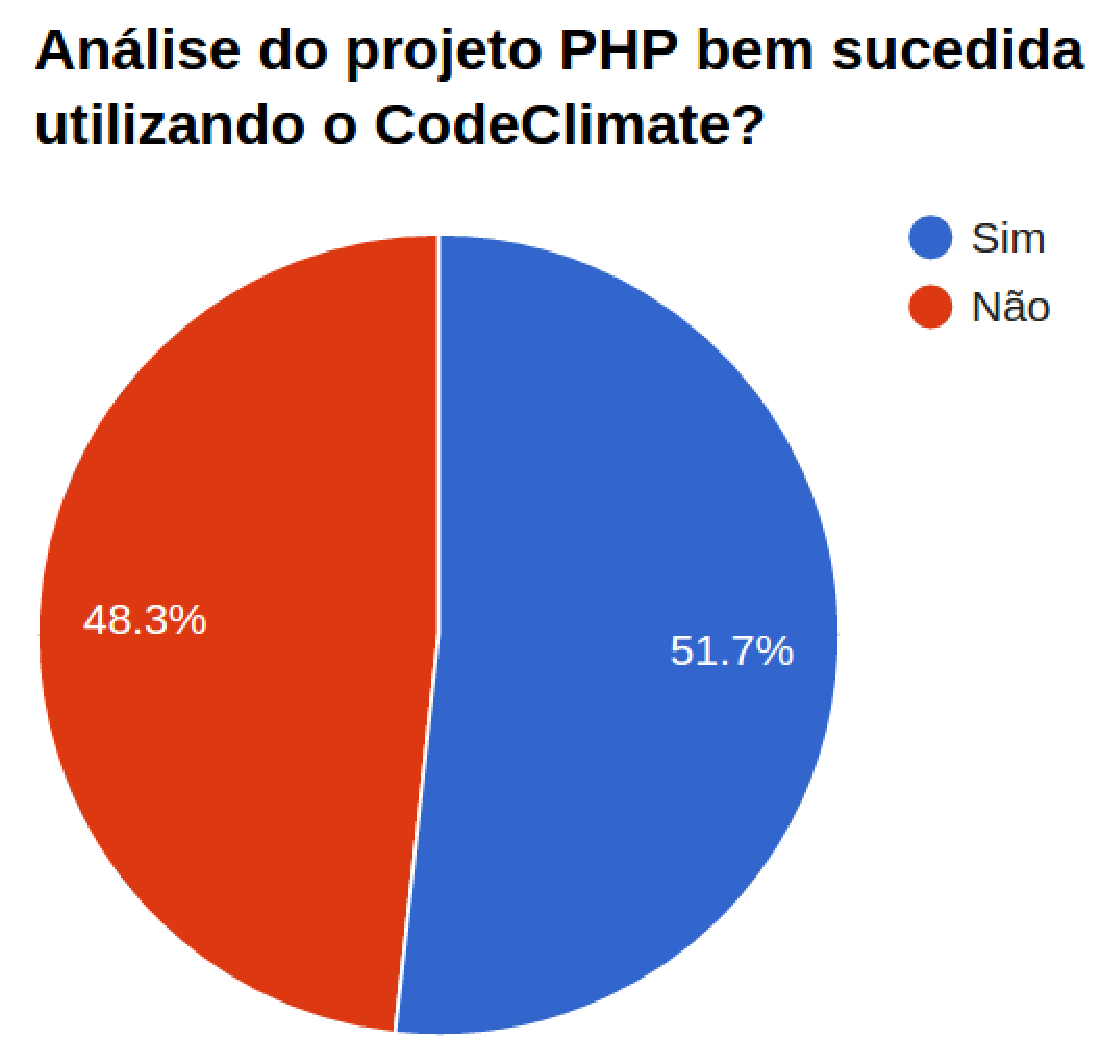
\includegraphics[keepaspectratio=true,scale=0.4]
    {figuras/is_codeclimate_php_success.eps}
  \caption{Porcentagens de Softwares com Análise bem sucedida no Code Climate}
  \label{fig:is_codeclimate_php_success}
\end{figure}

Foram adicionados 31 softwares do SPB em ambas as ferramentas (Mezuro e
Code Climate), desenvolvidos em PHP e Python. Estas adições resultaram na
análise descrita nos próximos parágrafos.
No Mezuro, dos 31 softwares adicionados, somente 4 obtiveram sucesso na
avaliação.

No Code Climate, 16 softwares realizaram a \textit{build} da avaliação com
sucesso. Nos que falharam, alguns dos erros foram encontrados em três das
\textit{engines}: ora em \textit{duplication}, ora na \textit{phpmd}, ora na
\textit{eslint}. E um dos processos gerou o erro 500. Em todas as falhas, é
sugerido ao usuário entrar em contato com o suporte da ferramenta. As falhas
são relacionadas com erros de \textit{time out}. A sugestão é a exclusão de
arquivos com bibliotecas de terceiros, \textit{assets} de produção (como
arquivos minimizados) e talvez arquivos de testes automatizados.

A Figura \ref{fig:is_codeclimate_php_success} mostra o percentual de sucesso na
análise dos projetos em PHP do SPB. Mais de 50\% conseguiram ter uma
\textit{build} bem sucedida, valor este que expõe, de certa forma, a baixa
qualidade dos softwares disponibilizados no SPB. Estes resultados da análise
exploratória demonstram que, em parte, os desafios encontrados na adição dos
projetos no Mezuro não estavam relacionados diretamente com o próprio Mezuro, e
sim com os projetos em PHP.

Considerando os motores e ferramentas utilizadas pelo Code Climate, pode-se
observar que nem todo projeto pode ser analisado por um conjunto de métricas ou
definições de estilo pré estabelecida. Fato este que intensifica a utilização do
Mezuro em que o usuário é capaz de criar as Configurações com o conjunto de
métricas que desejar, adaptando assim ao seu projeto. Portanto, se não há um
conjunto fechado ideal para todo projeto, é possível afirmar que também não há
uma visualização única para todas as Configurações ou conjunto de métricas.

Adicionalmente, também foram inseridos no Mezuro para avaliação, 5 projetos dos
17 desenvolvidos em Java, com o intuito de ser um contraponto ao Code Climate
por esta não compreender a análise de projetos em Java, C, ou C++. Infelizmente
nenhuma das \textit{builds} resultou em resultados concretos.

\newpage

\begin{figure}[!htb]
	\centering
    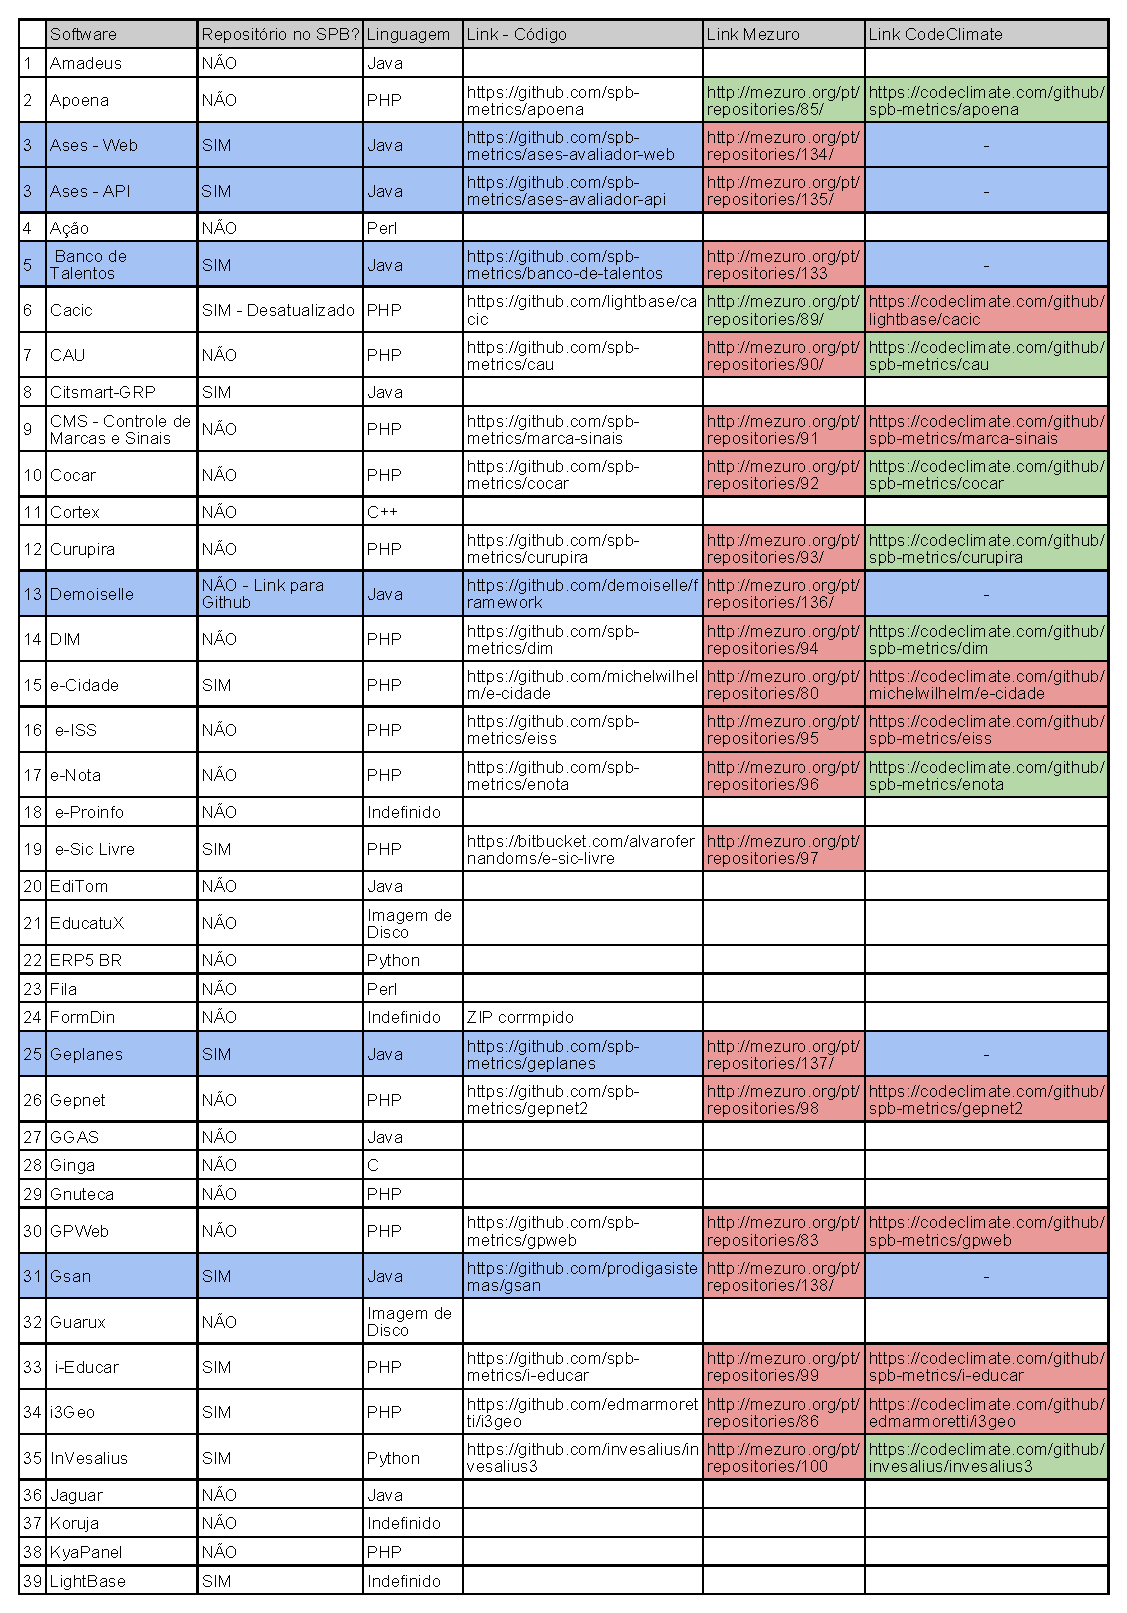
\includegraphics[keepaspectratio=true,scale=0.85]
    {tabelas/spb_1_v2-crop.eps}
  \caption{Categorização - Softwares SPB - Parte 1}
  \label{fig:softwares_spb_1}
\end{figure}

\newpage

\begin{figure}[!htb]
	\centering
    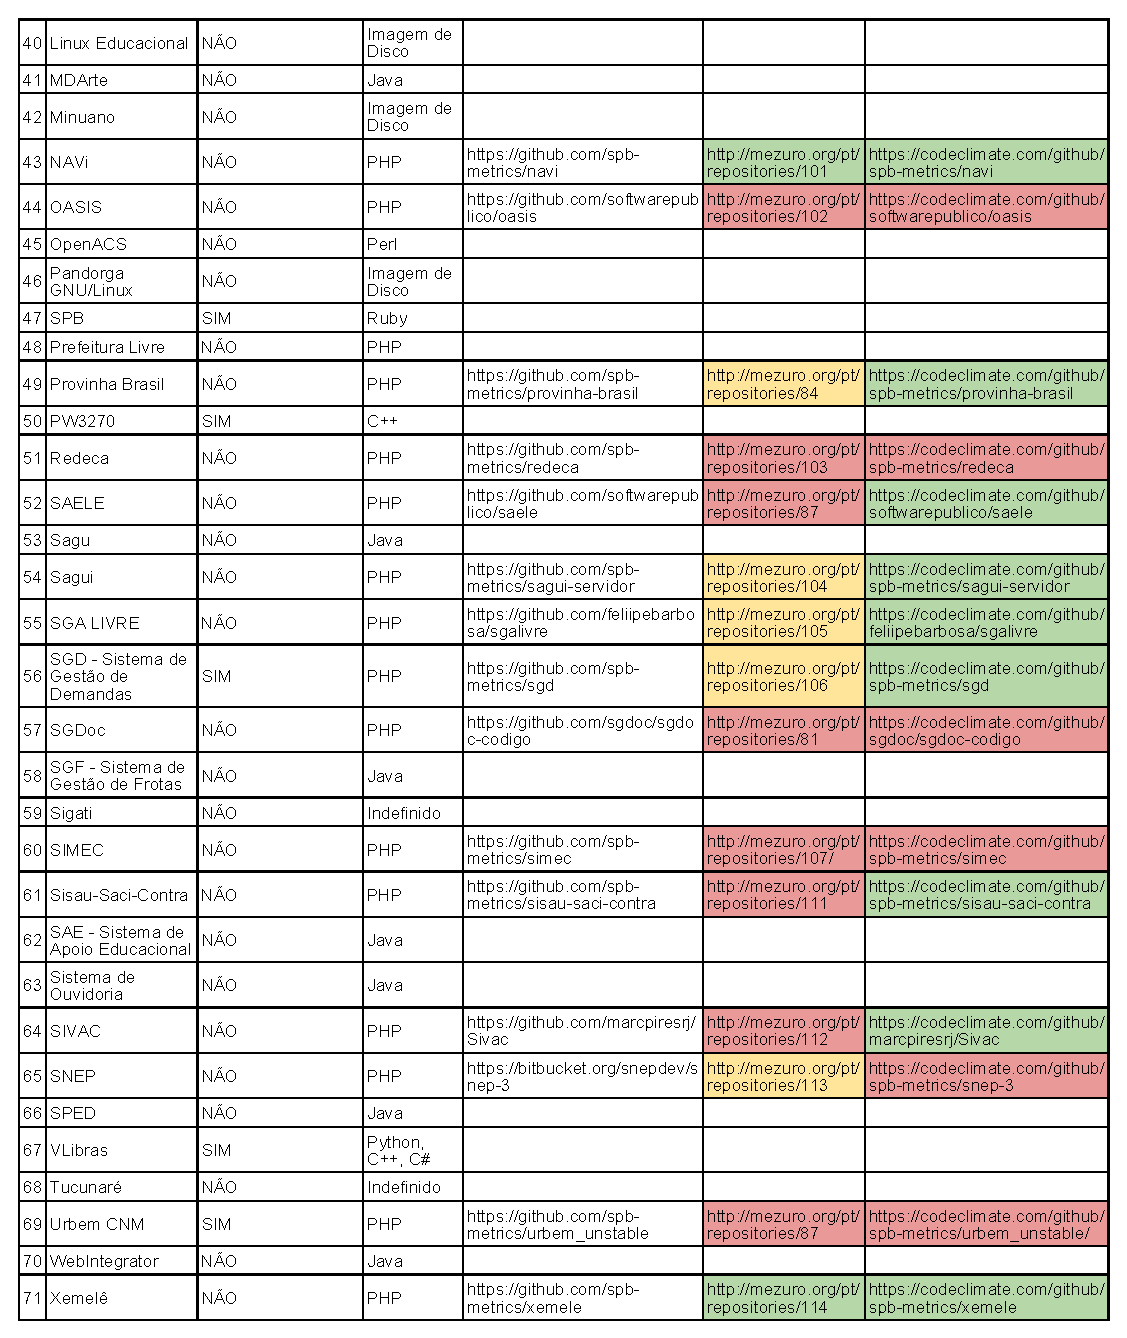
\includegraphics[keepaspectratio=true,scale=0.85]
    {tabelas/spb_2_v2-crop.eps}
  \caption{Categorização - Softwares SPB - Parte 2}
  \label{fig:softwares_spb_2}
\end{figure}

\newpage

As tabelas das Figuras \ref{fig:softwares_spb_1} e \ref{fig:softwares_spb_2}
mostram a categorização dos softwares do SPB.
As cores de fundo das colunas ``Link Mezuro'' e ``Link CodeClimate'',
representam o resultado das análises realizadas por estas ferramentas. Se verde,
a análise foi realizada com sucesso. Se amarelo, a análise foi concluída, porém
as métricas não foram carregadas. E quando o fundo é vermelho, a análise não
obteve êxito. As linhas que estão destacadas com o fundo azul são os projetos em
Java que foram adicionados ao Mezuro.

\section{Exemplo da Análise por Projeto: Xemelê}

O Xemelê\footnote{\url{https://softwarepublico.gov.br/social/xemele}} é um
software para o gerenciamento de ambientes integrados com sites, blogs, chats,
\textit{wikis} e e-mails. Desenvolvido na linguagem de programação PHP e
utilizando outros recursos, como HTML, Javascript, jQuery e banco de dados MySQL.

A análise realizada pelo Mezuro desta ferramenta, retornou a nota zero para o
projeto como um todo. E a métrica de destaque, relacionada com o arquivo
\textbf{functions.php} da raiz do projeto, está relacionada com o método
\textbf{recent\_comments} em que é recomendado a remoção da expressão
\textit{else} da linha 52 e a simplificação do código para trabalhar sem esta
expressão de condição. Link para a avaliação no Mezuro
\footnote{\url{http://mezuro.org/pt/repositories/114}}.

Já a nota dada ao projeto pelo Code Climate foi a de 2.18/4. E os arquivos com
notas \textbf{F} e \textbf{D} são os arquivos Javascript \textit{js/jquery.cycle.js}
e \textit{js/jquery.js}, respectivamente. Além disso, a ferramenta mostra para o
usuário 4 páginas de possíveis problemas encontrados, nas diversas categorias,
tais como, problemas com complexidade, duplicação de código, estilo nos arquivos
CSS, clareza, possíveis ou risco de \textit{bugs} e problemas com compatibilidade. E o
mesmo destaque dado ao arquivo \textbf{functions.php} pelo Mezuro, também foi
destacado no Code Climate, mesmo assim, foi atribuído a maior nota possível, nota
\textbf{A}. Por fim, é destacado que as \textit{engines} que apontaram estes possíveis
erros são: \textit{csslint}, \textit{duplication}, \textit{eslint} e
\textit{phpmd} Link para a avaliação no Code Climate
\footnote{\url{https://codeclimate.com/github/spb-metrics/xemele}}.

\begin{figure}[!htb]
	\centering
    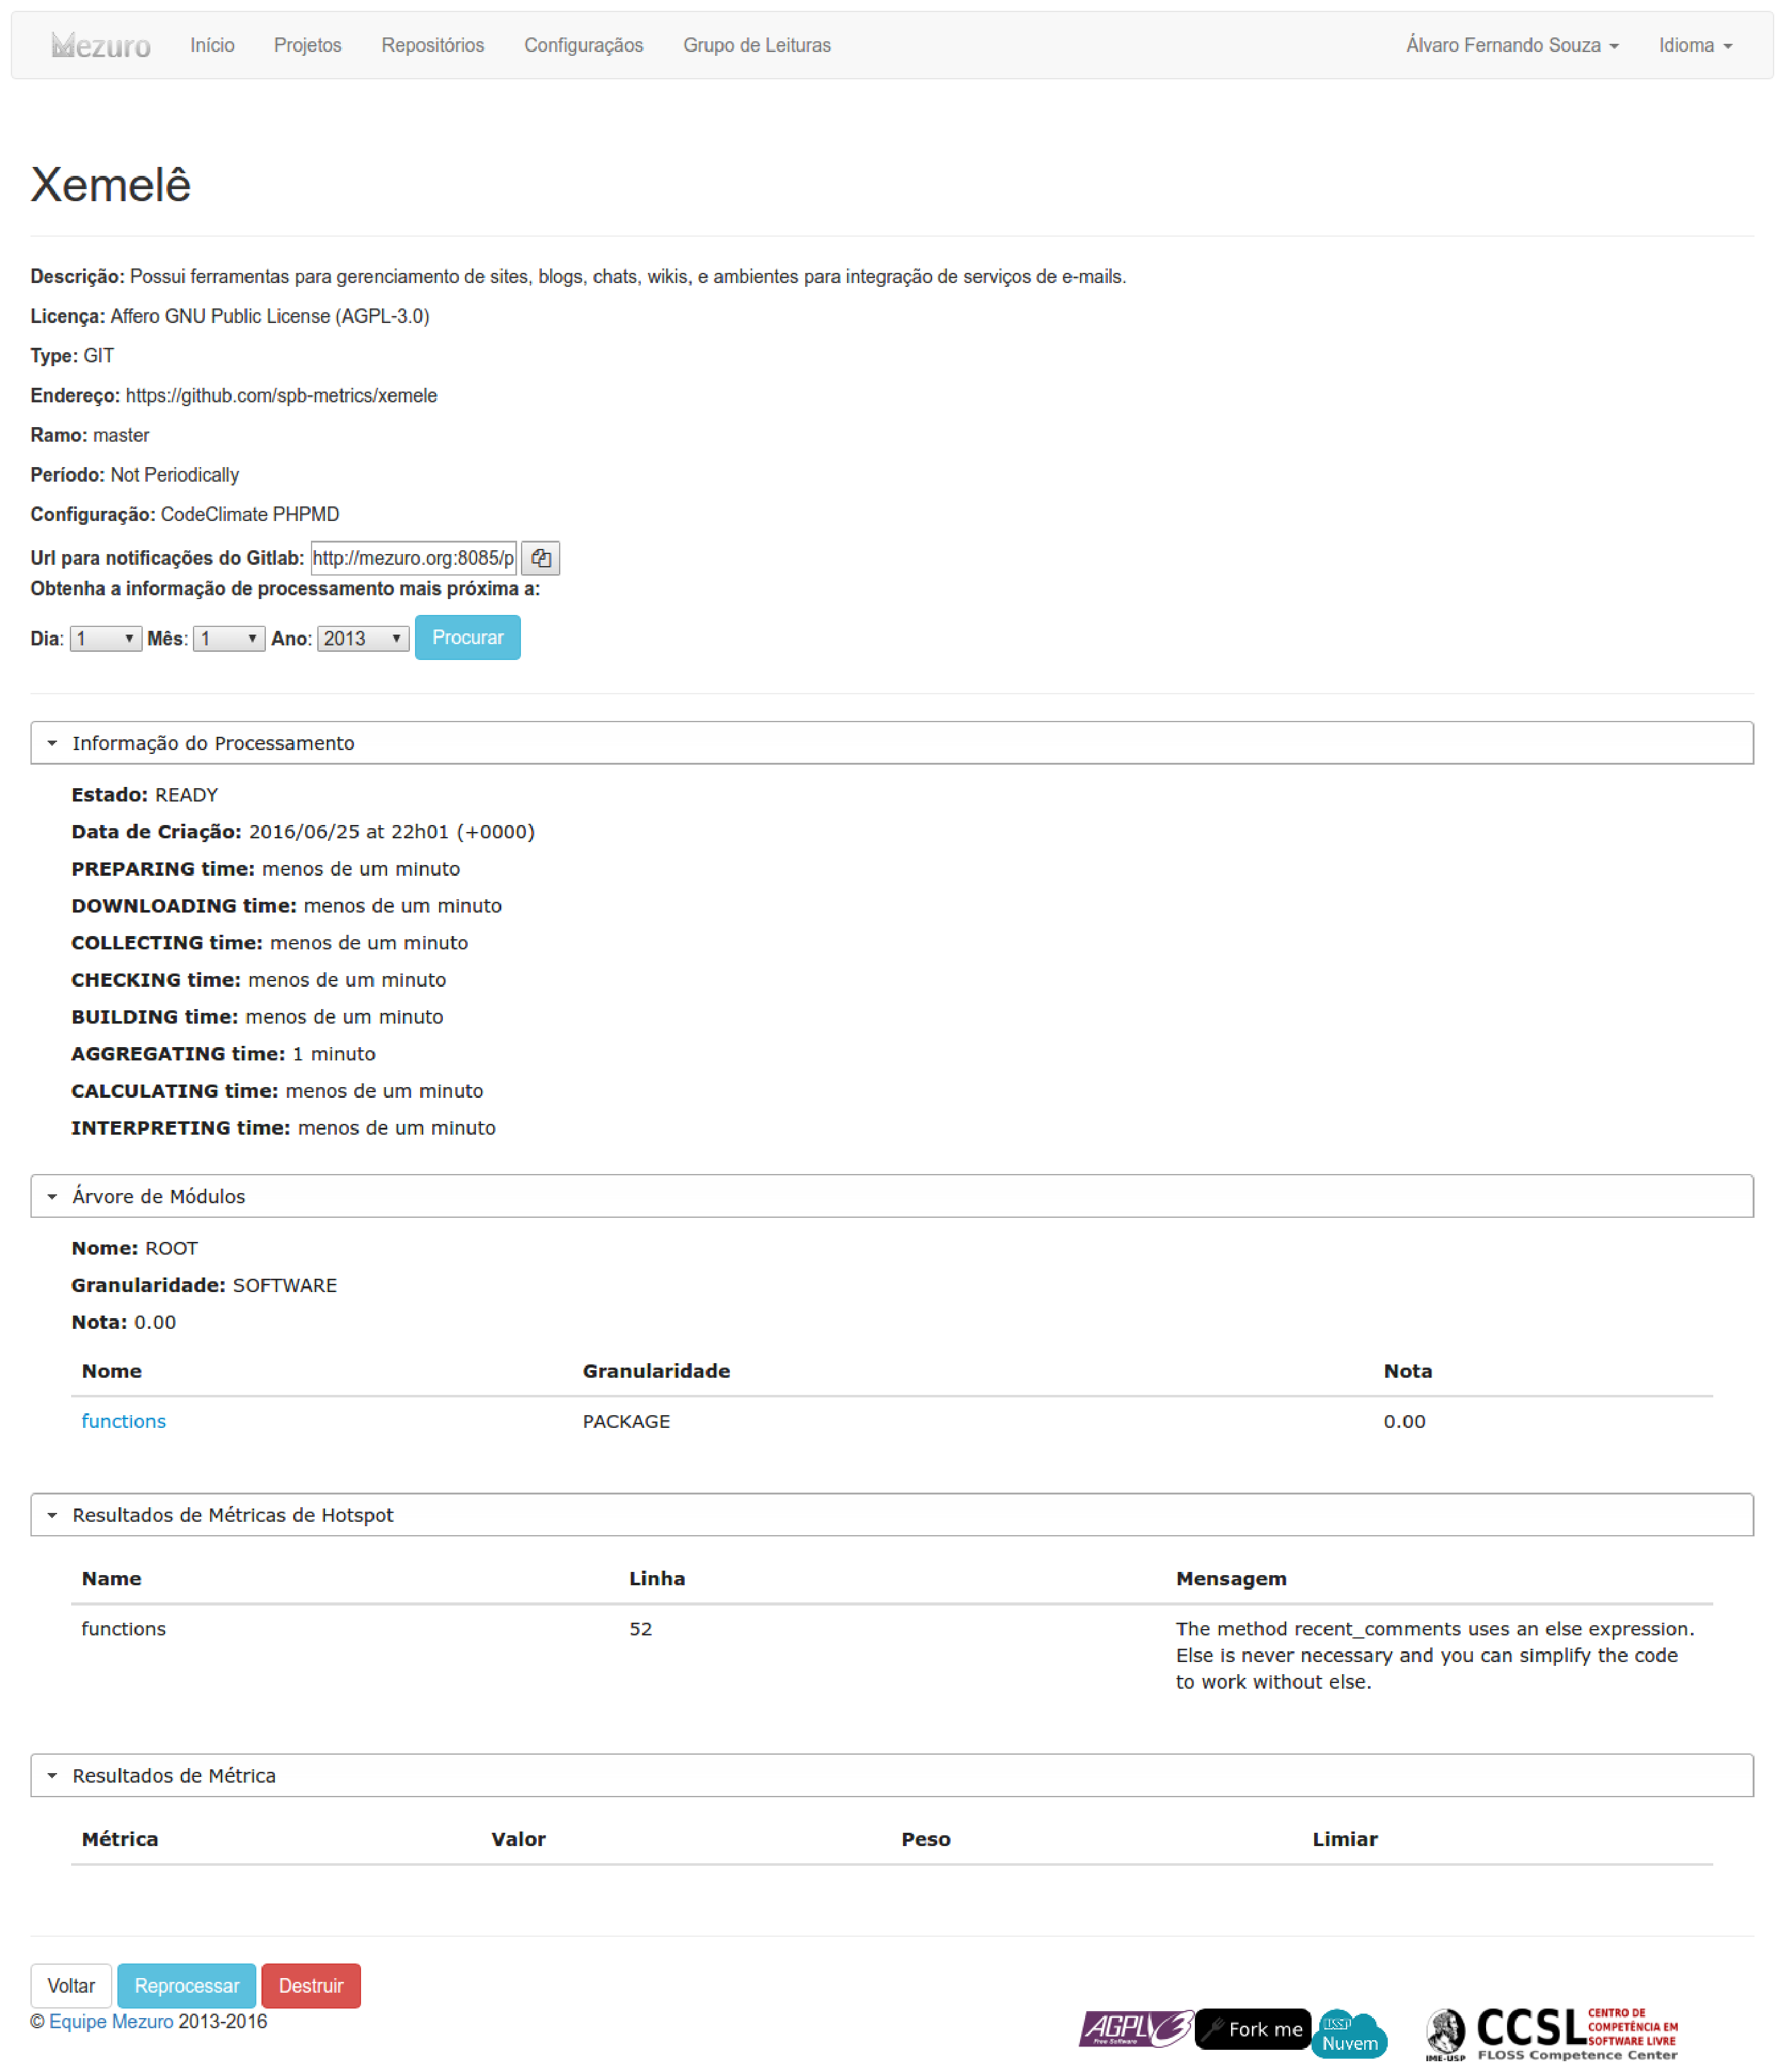
\includegraphics[keepaspectratio=true,scale=0.3]
    {figuras/mezuro-repositorio-view.eps}
  \caption{Mezuro - Página de Repositório}
	\label{fig:mezuro-repositorio-view-xemele}
\end{figure}

A Figura \ref{fig:mezuro-repositorio-view-xemele}
mostra os resultados da análise\footnote{\url{http://mezuro.org/pt/repositories/114}}
de um dos softwares do SPB, o Xemelê.

\newpage

\begin{figure}[!htb]
	\centering
    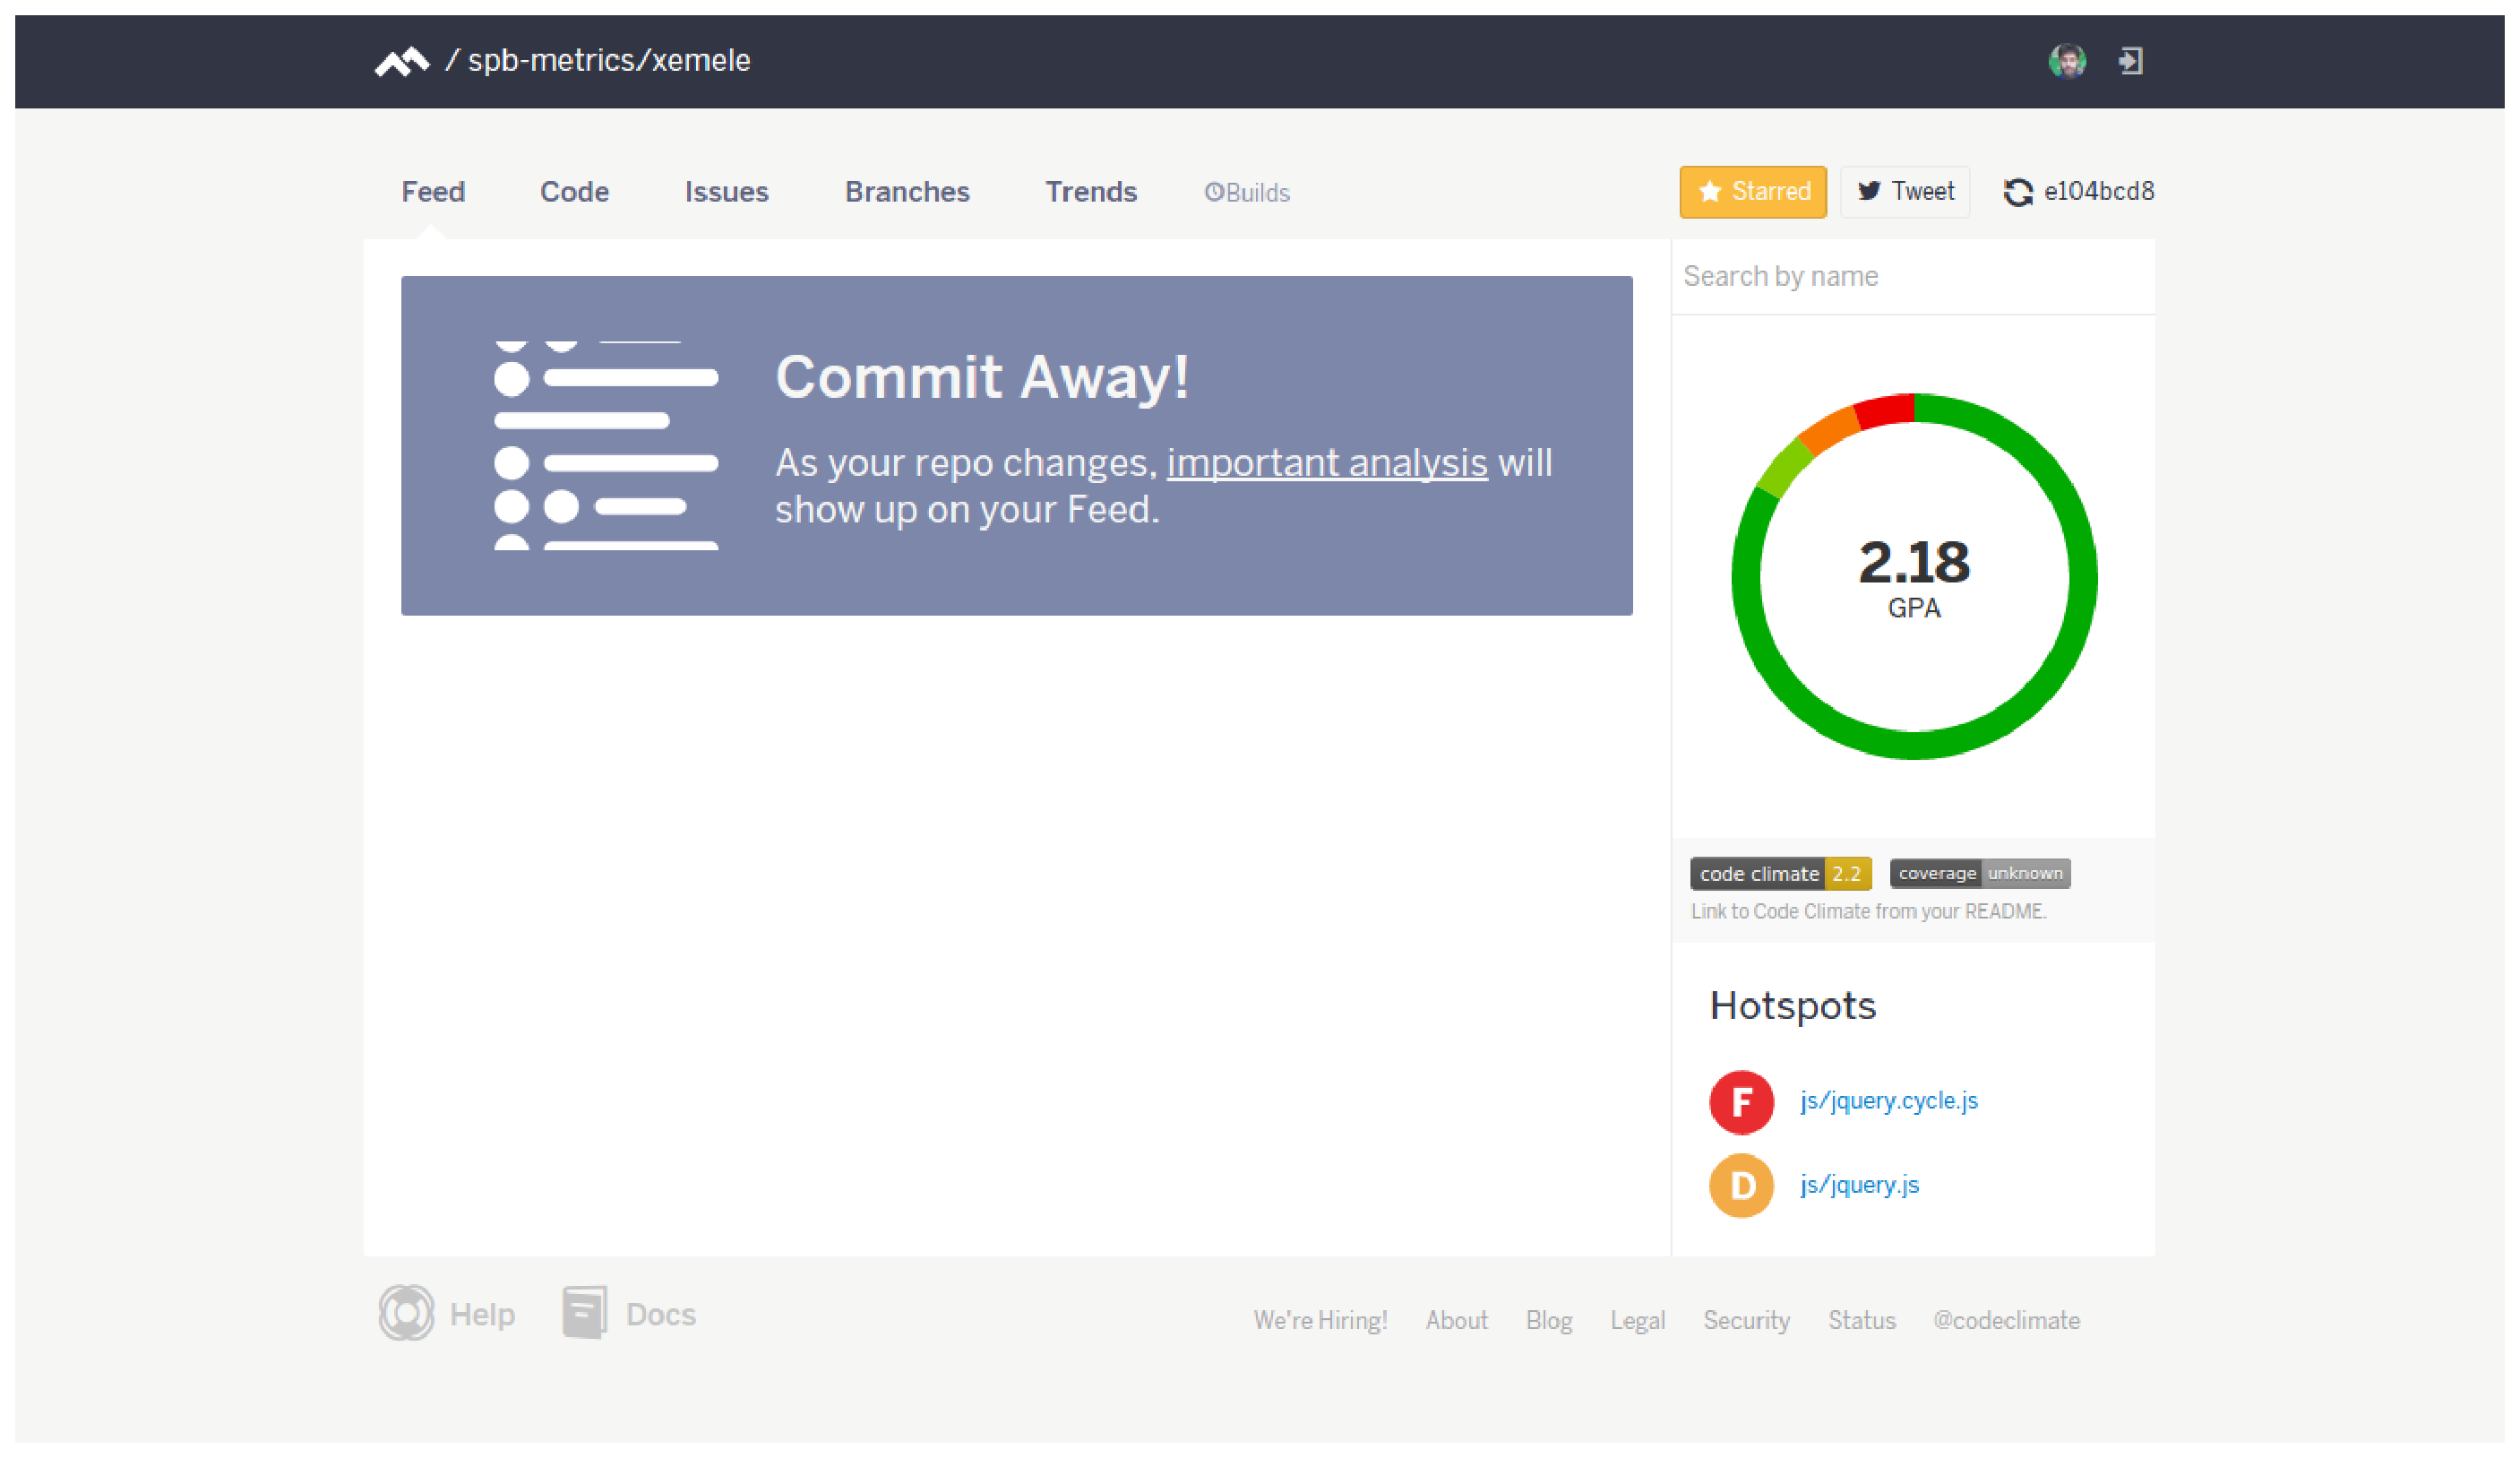
\includegraphics[keepaspectratio=true,scale=0.35]
    {figuras/codeclimate_feed.eps}
  \caption{Code Climate - Xemelê - Aba \textit{Feed}}
	\label{fig:codeclimate_feed}
\end{figure}

\begin{figure}[!htb]
	\centering
    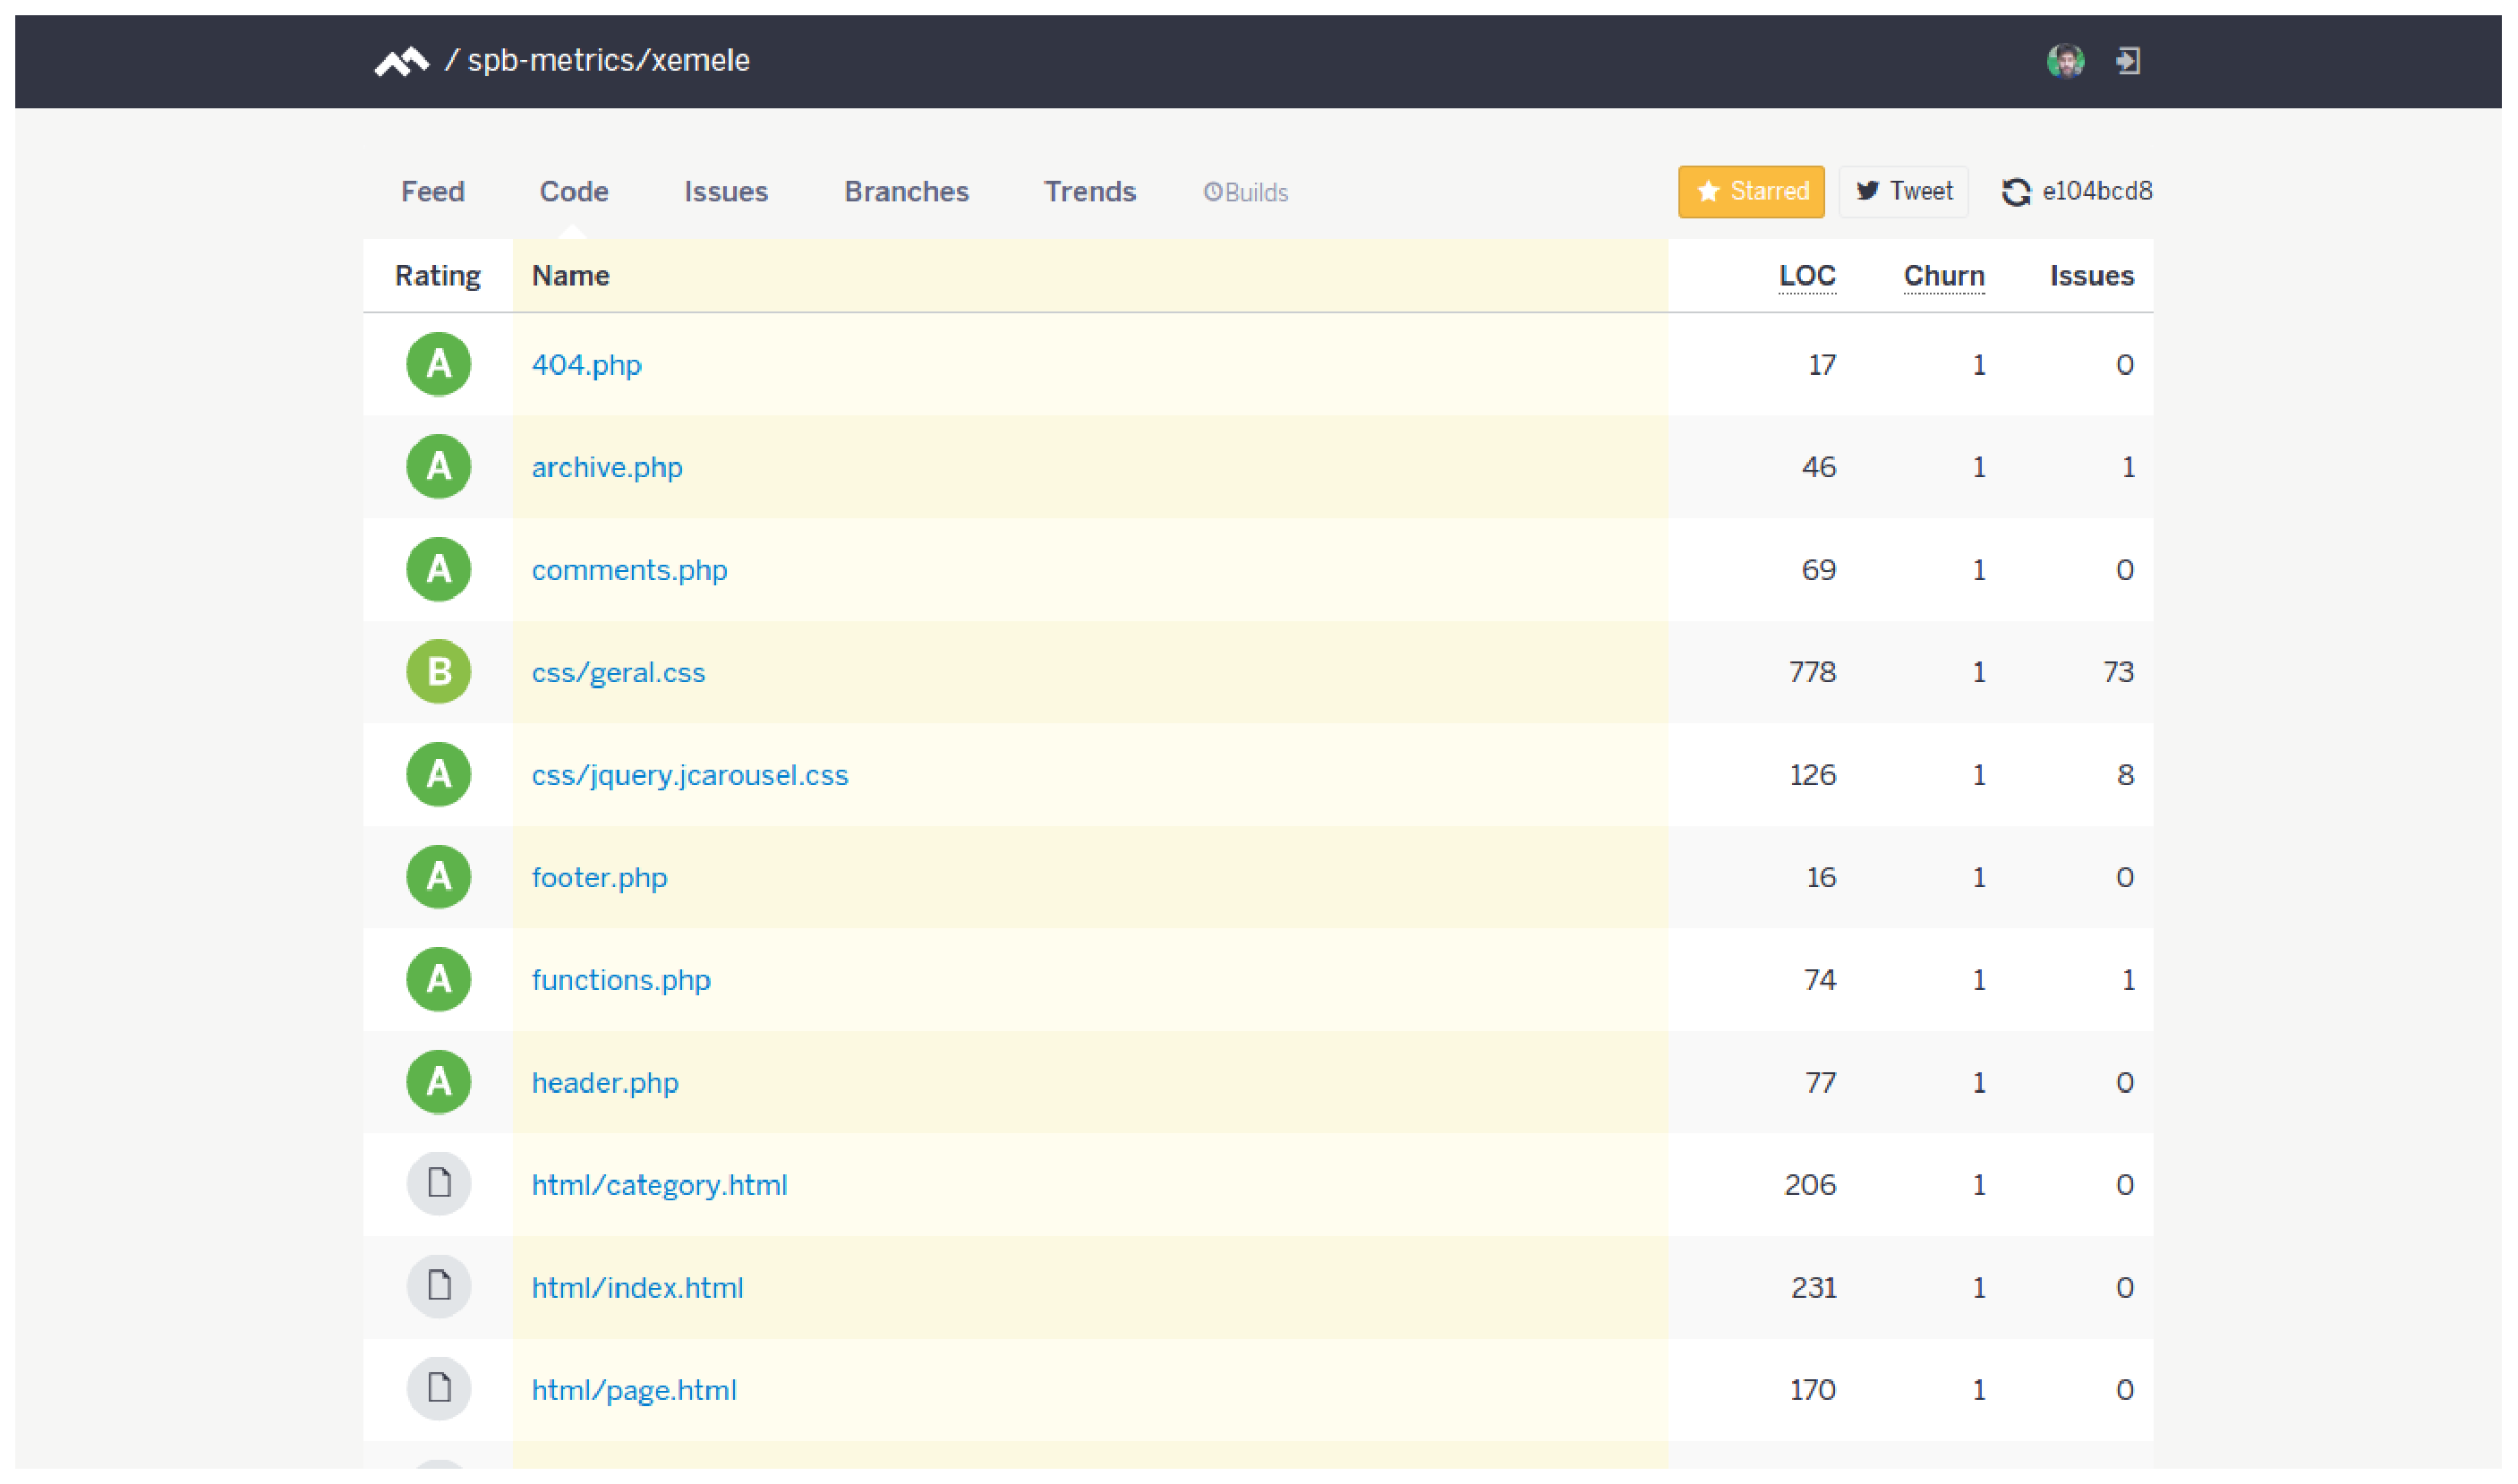
\includegraphics[keepaspectratio=true,scale=0.35]
    {figuras/codeclimate_code_tab.eps}
  \caption{Code Climate - Xemelê - Aba \textit{Code} (parcial)}
	\label{fig:codeclimate_code_tab}
\end{figure}

\newpage

\begin{figure}[!htb]
	\centering
    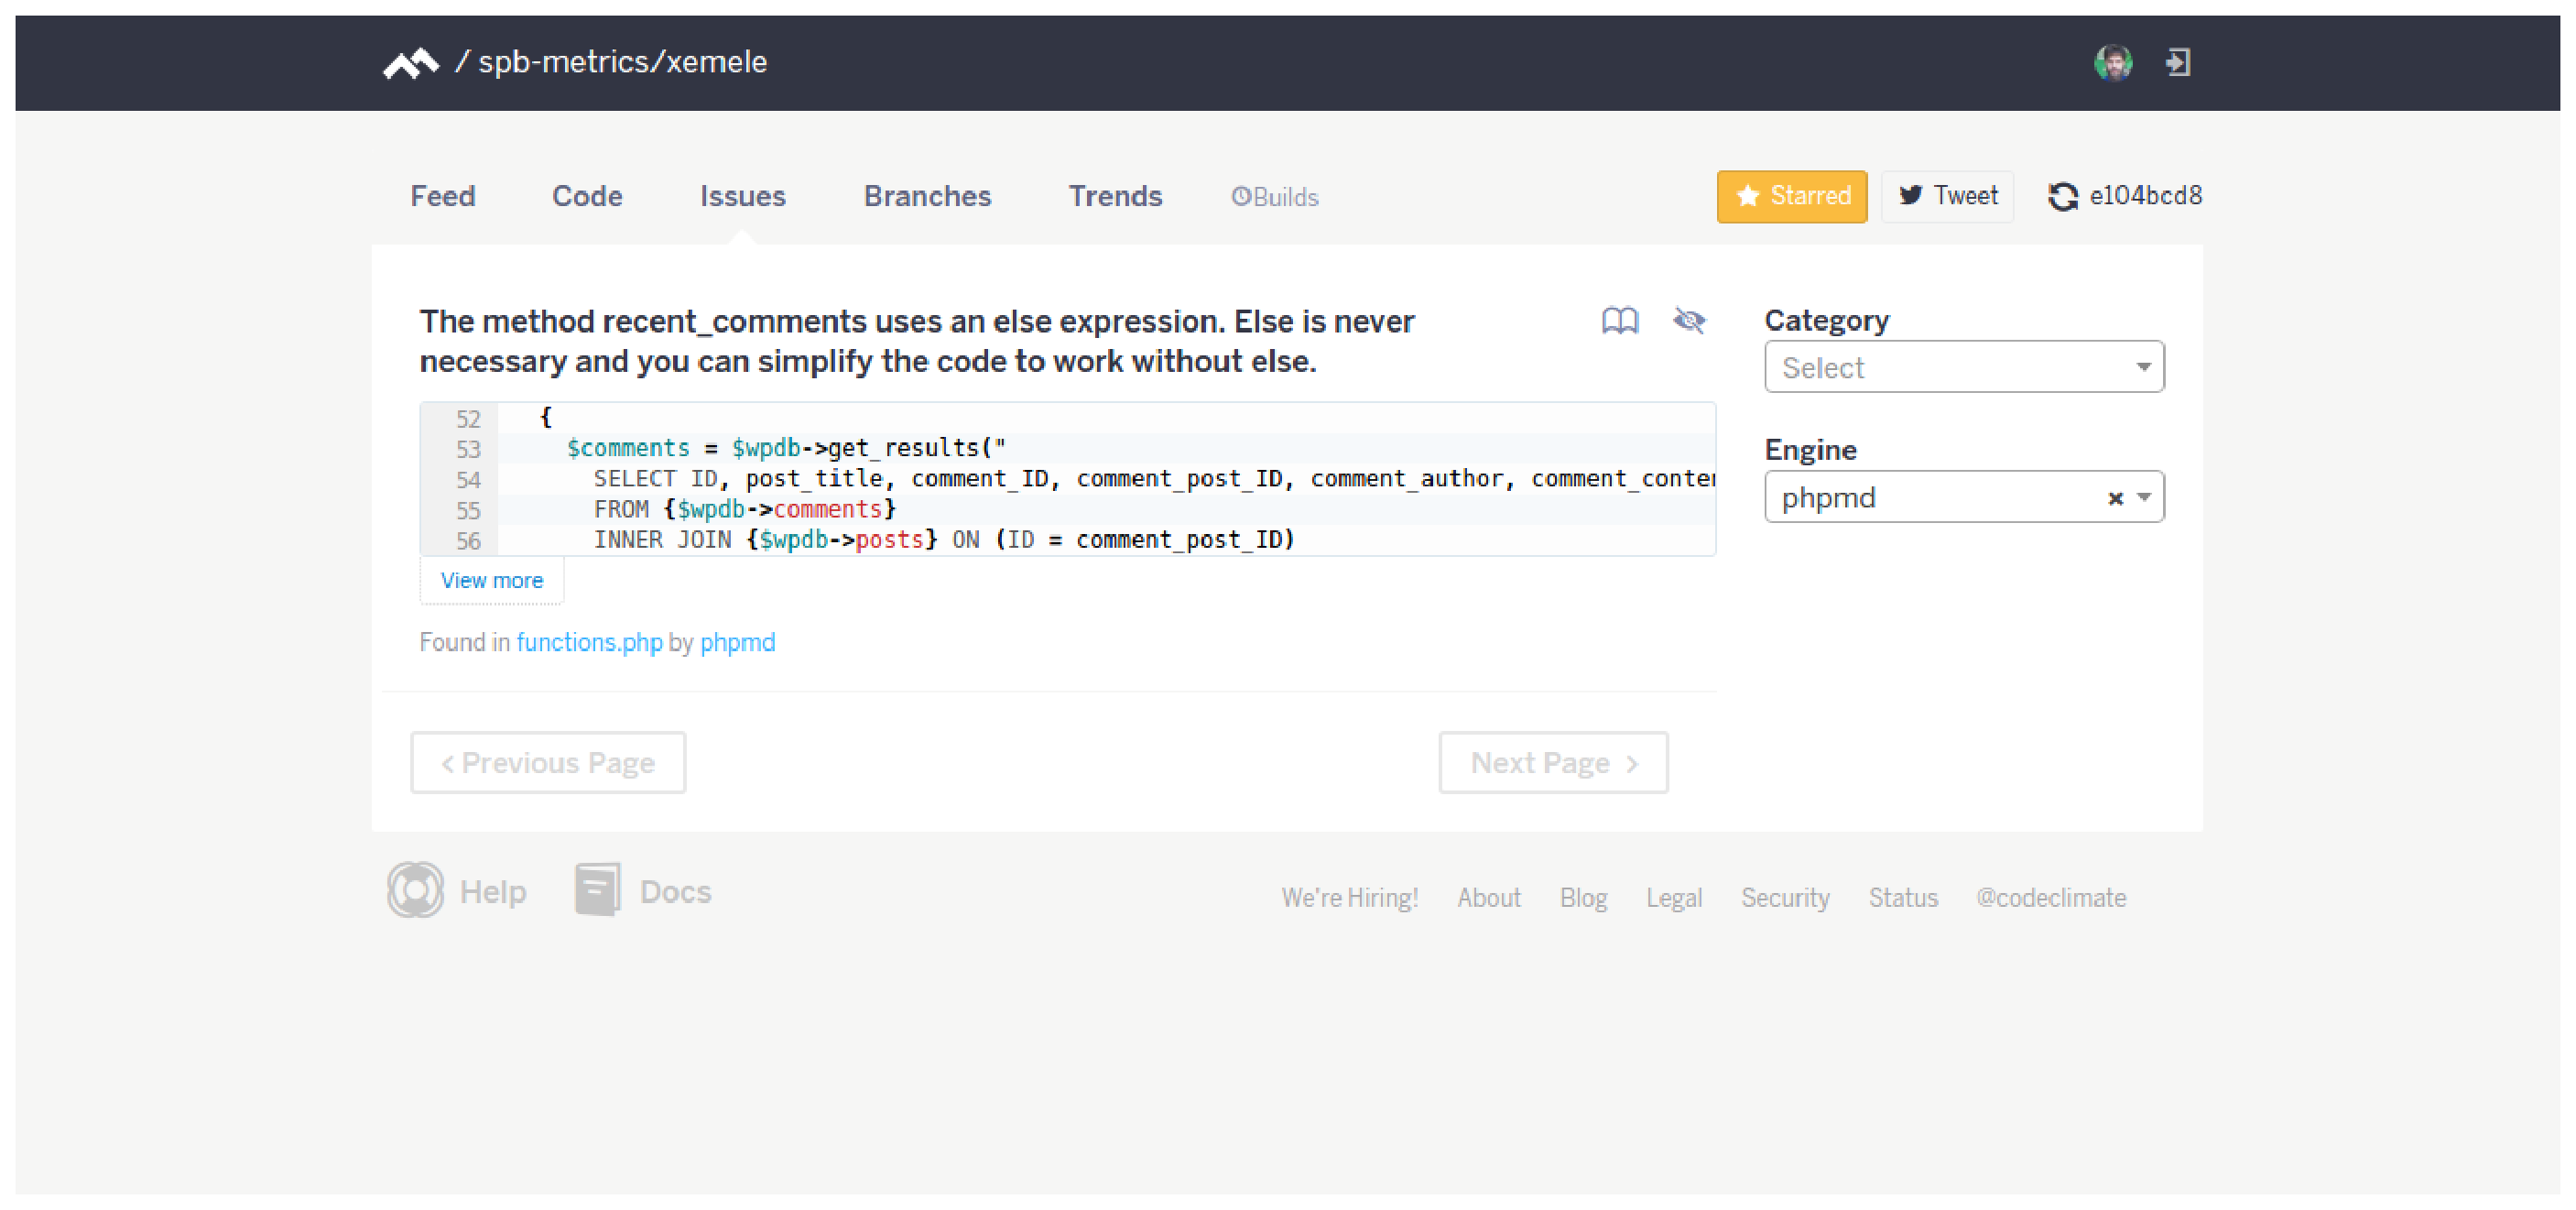
\includegraphics[keepaspectratio=true,scale=0.35]
    {figuras/codeclimate_issues_tab_phpmd.eps}
  \caption{Code Climate - Xemelê - Aba \textit{Issues} (PHPMD)}
	\label{fig:codeclimate_issues_tab_phpmd}
\end{figure}

\begin{figure}[!htb]
	\centering
    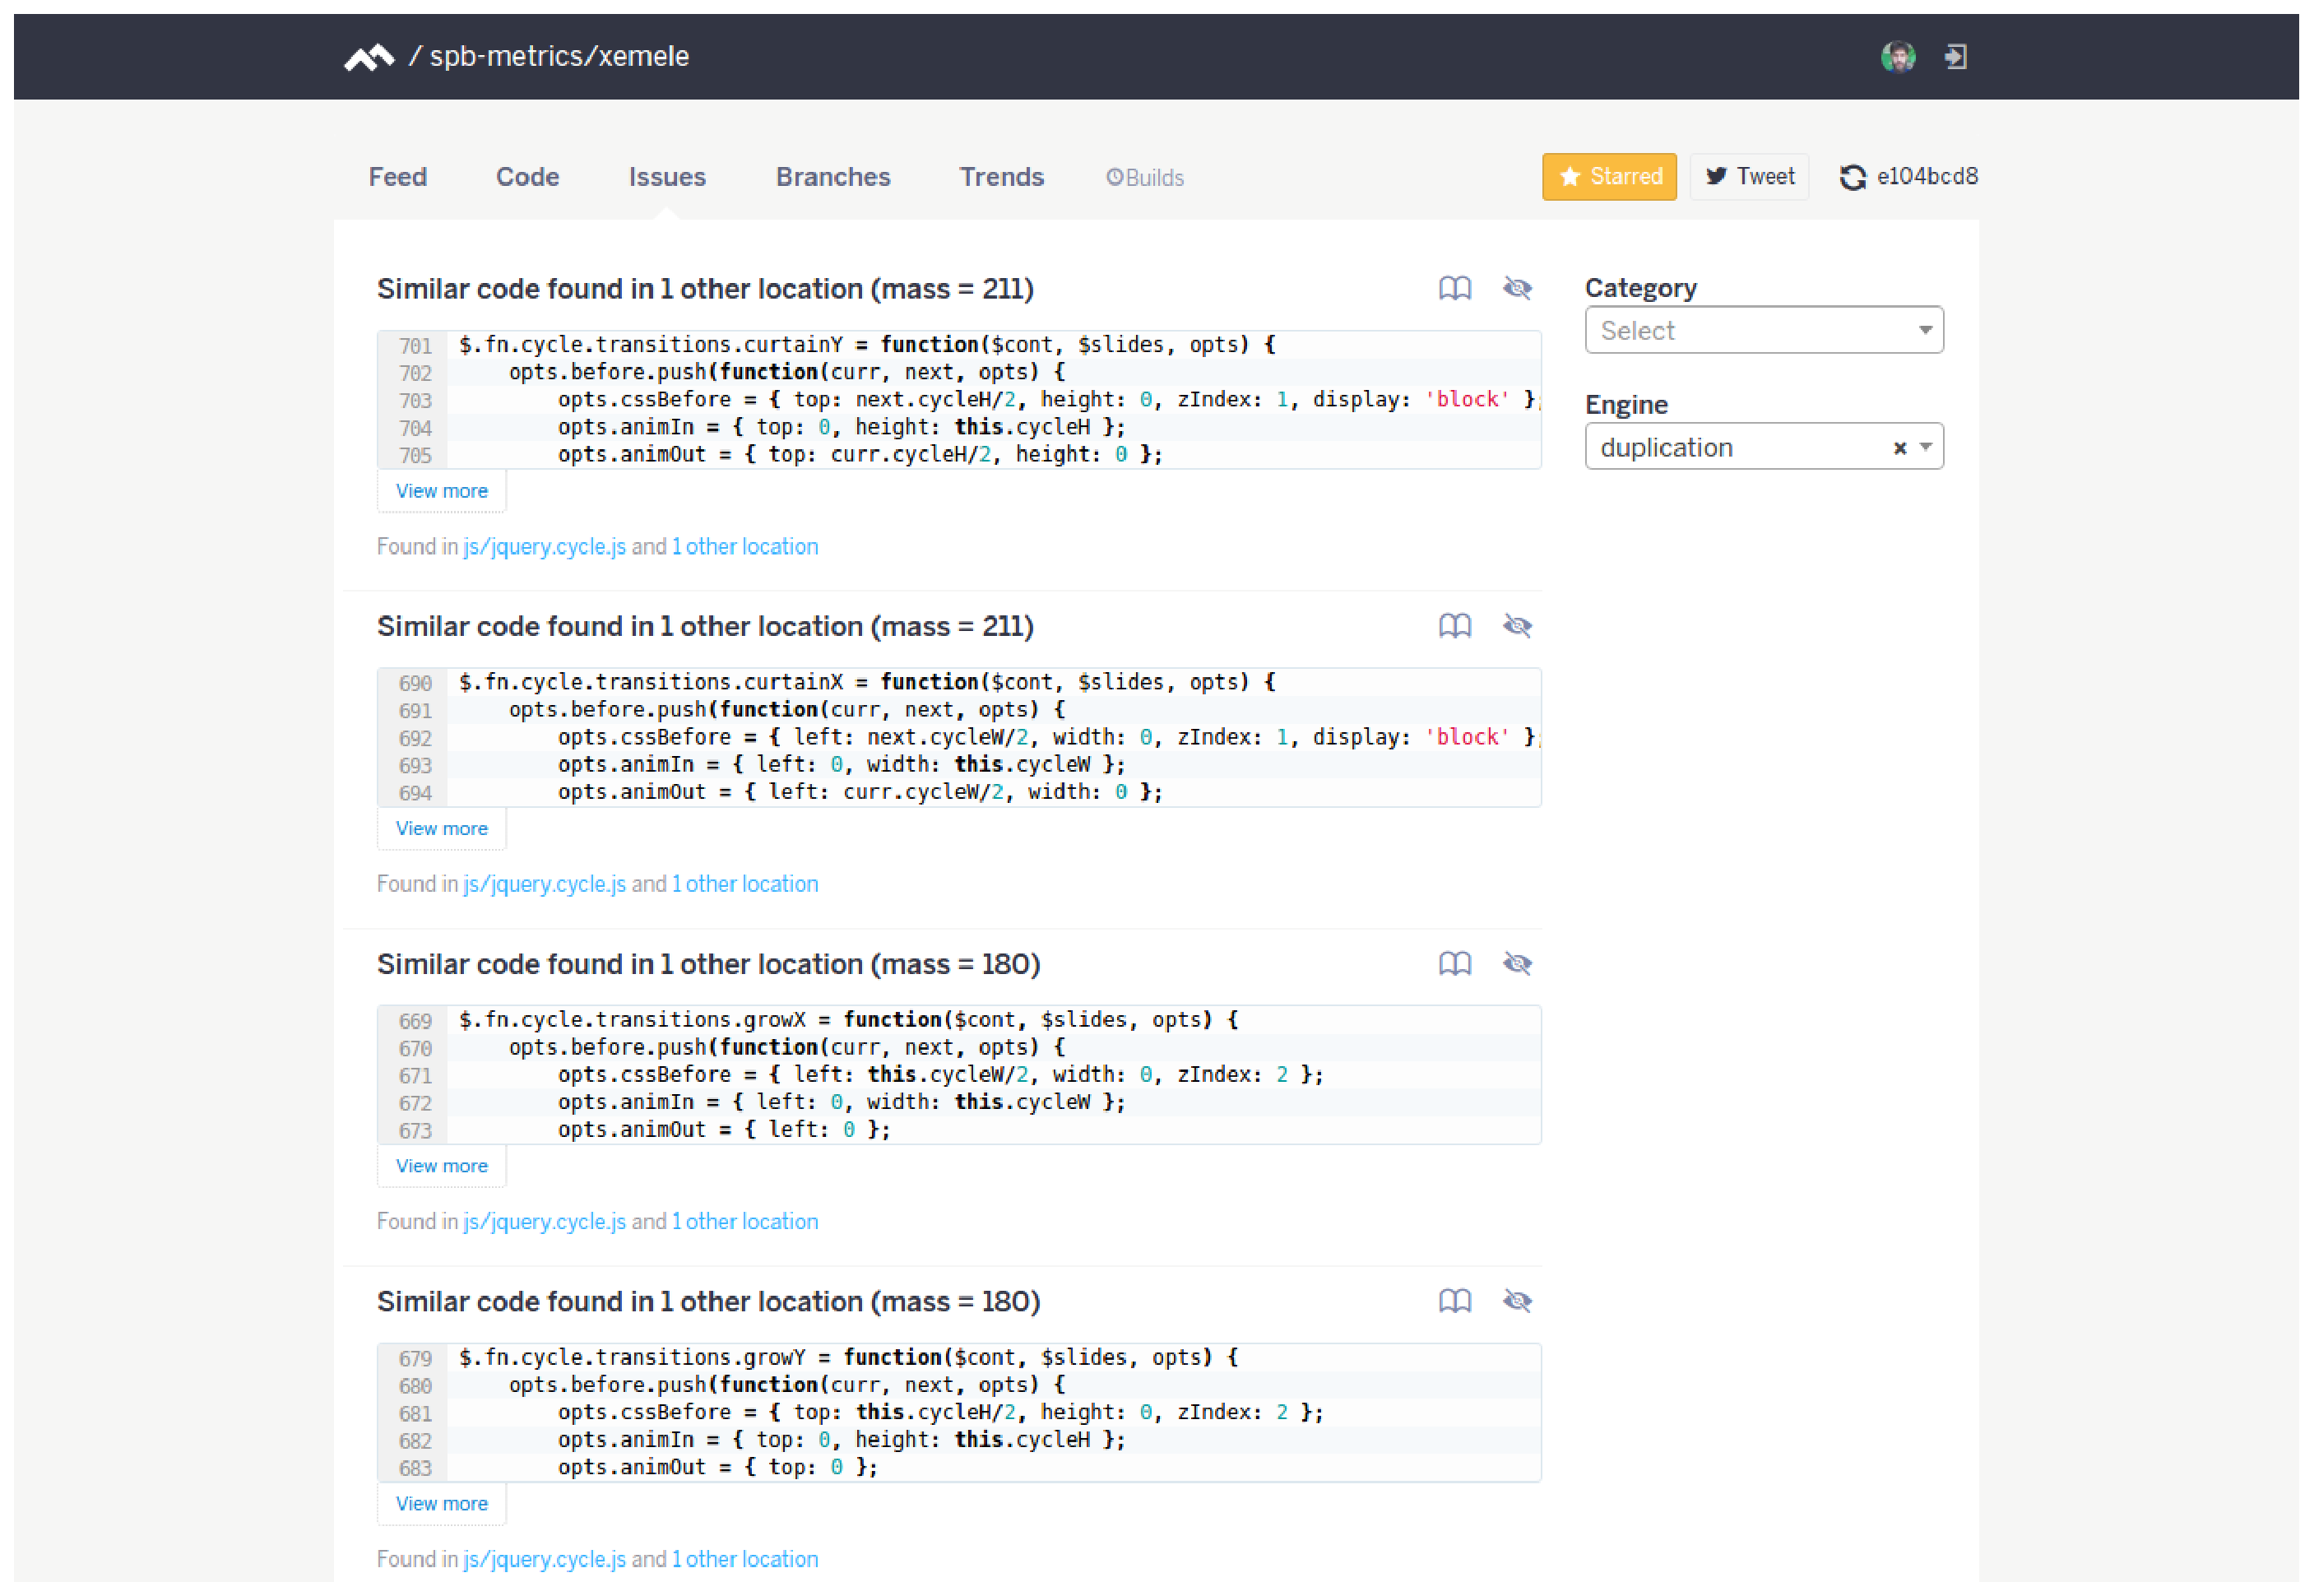
\includegraphics[keepaspectratio=true,scale=0.35]
    {figuras/codeclimate_issues_tab_duplication.eps}
  \caption{Code Climate - Xemelê - Aba \textit{Issues} (Duplication)}
	\label{fig:codeclimate_issues_tab_duplication}
\end{figure}

\newpage

\begin{figure}[!htb]
	\centering
    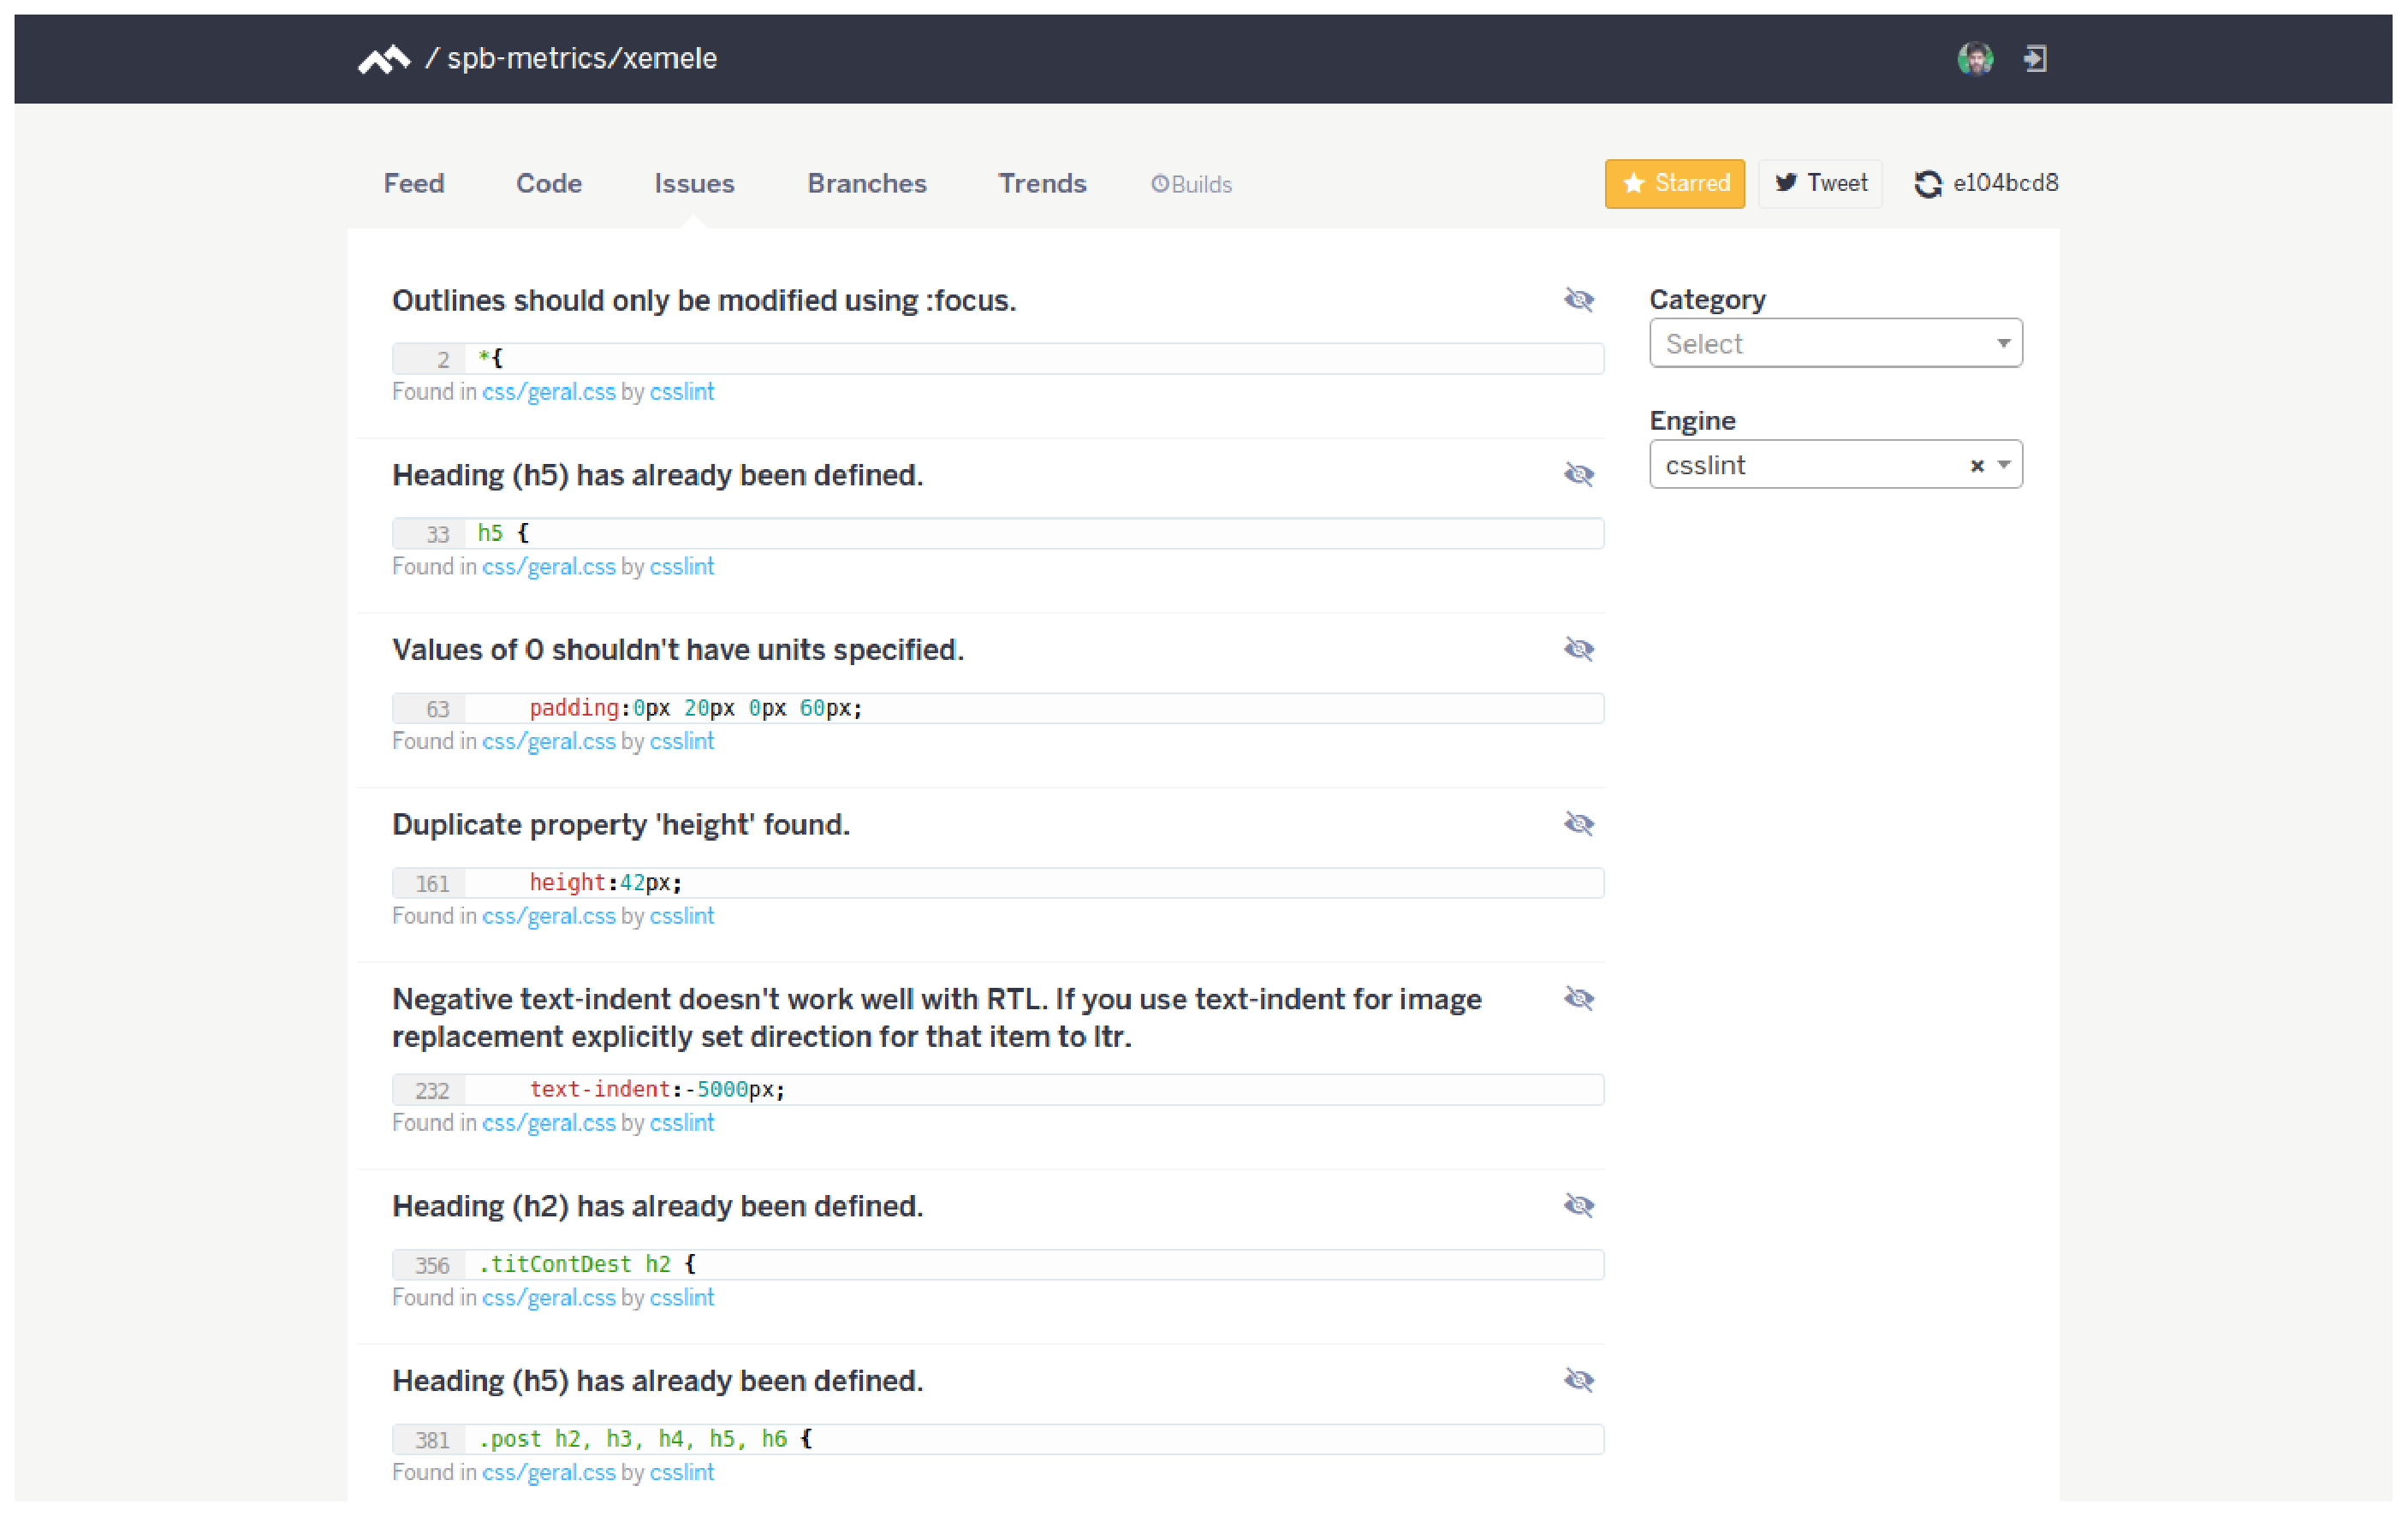
\includegraphics[keepaspectratio=true,scale=0.35]
    {figuras/codeclimate_issues_tab_csslint.eps}
  \caption{Code Climate - Xemelê - Aba \textit{Issues} (CSSLint)}
	\label{fig:codeclimate_issues_tab_csslint}
\end{figure}

\begin{figure}[!htb]
	\centering
    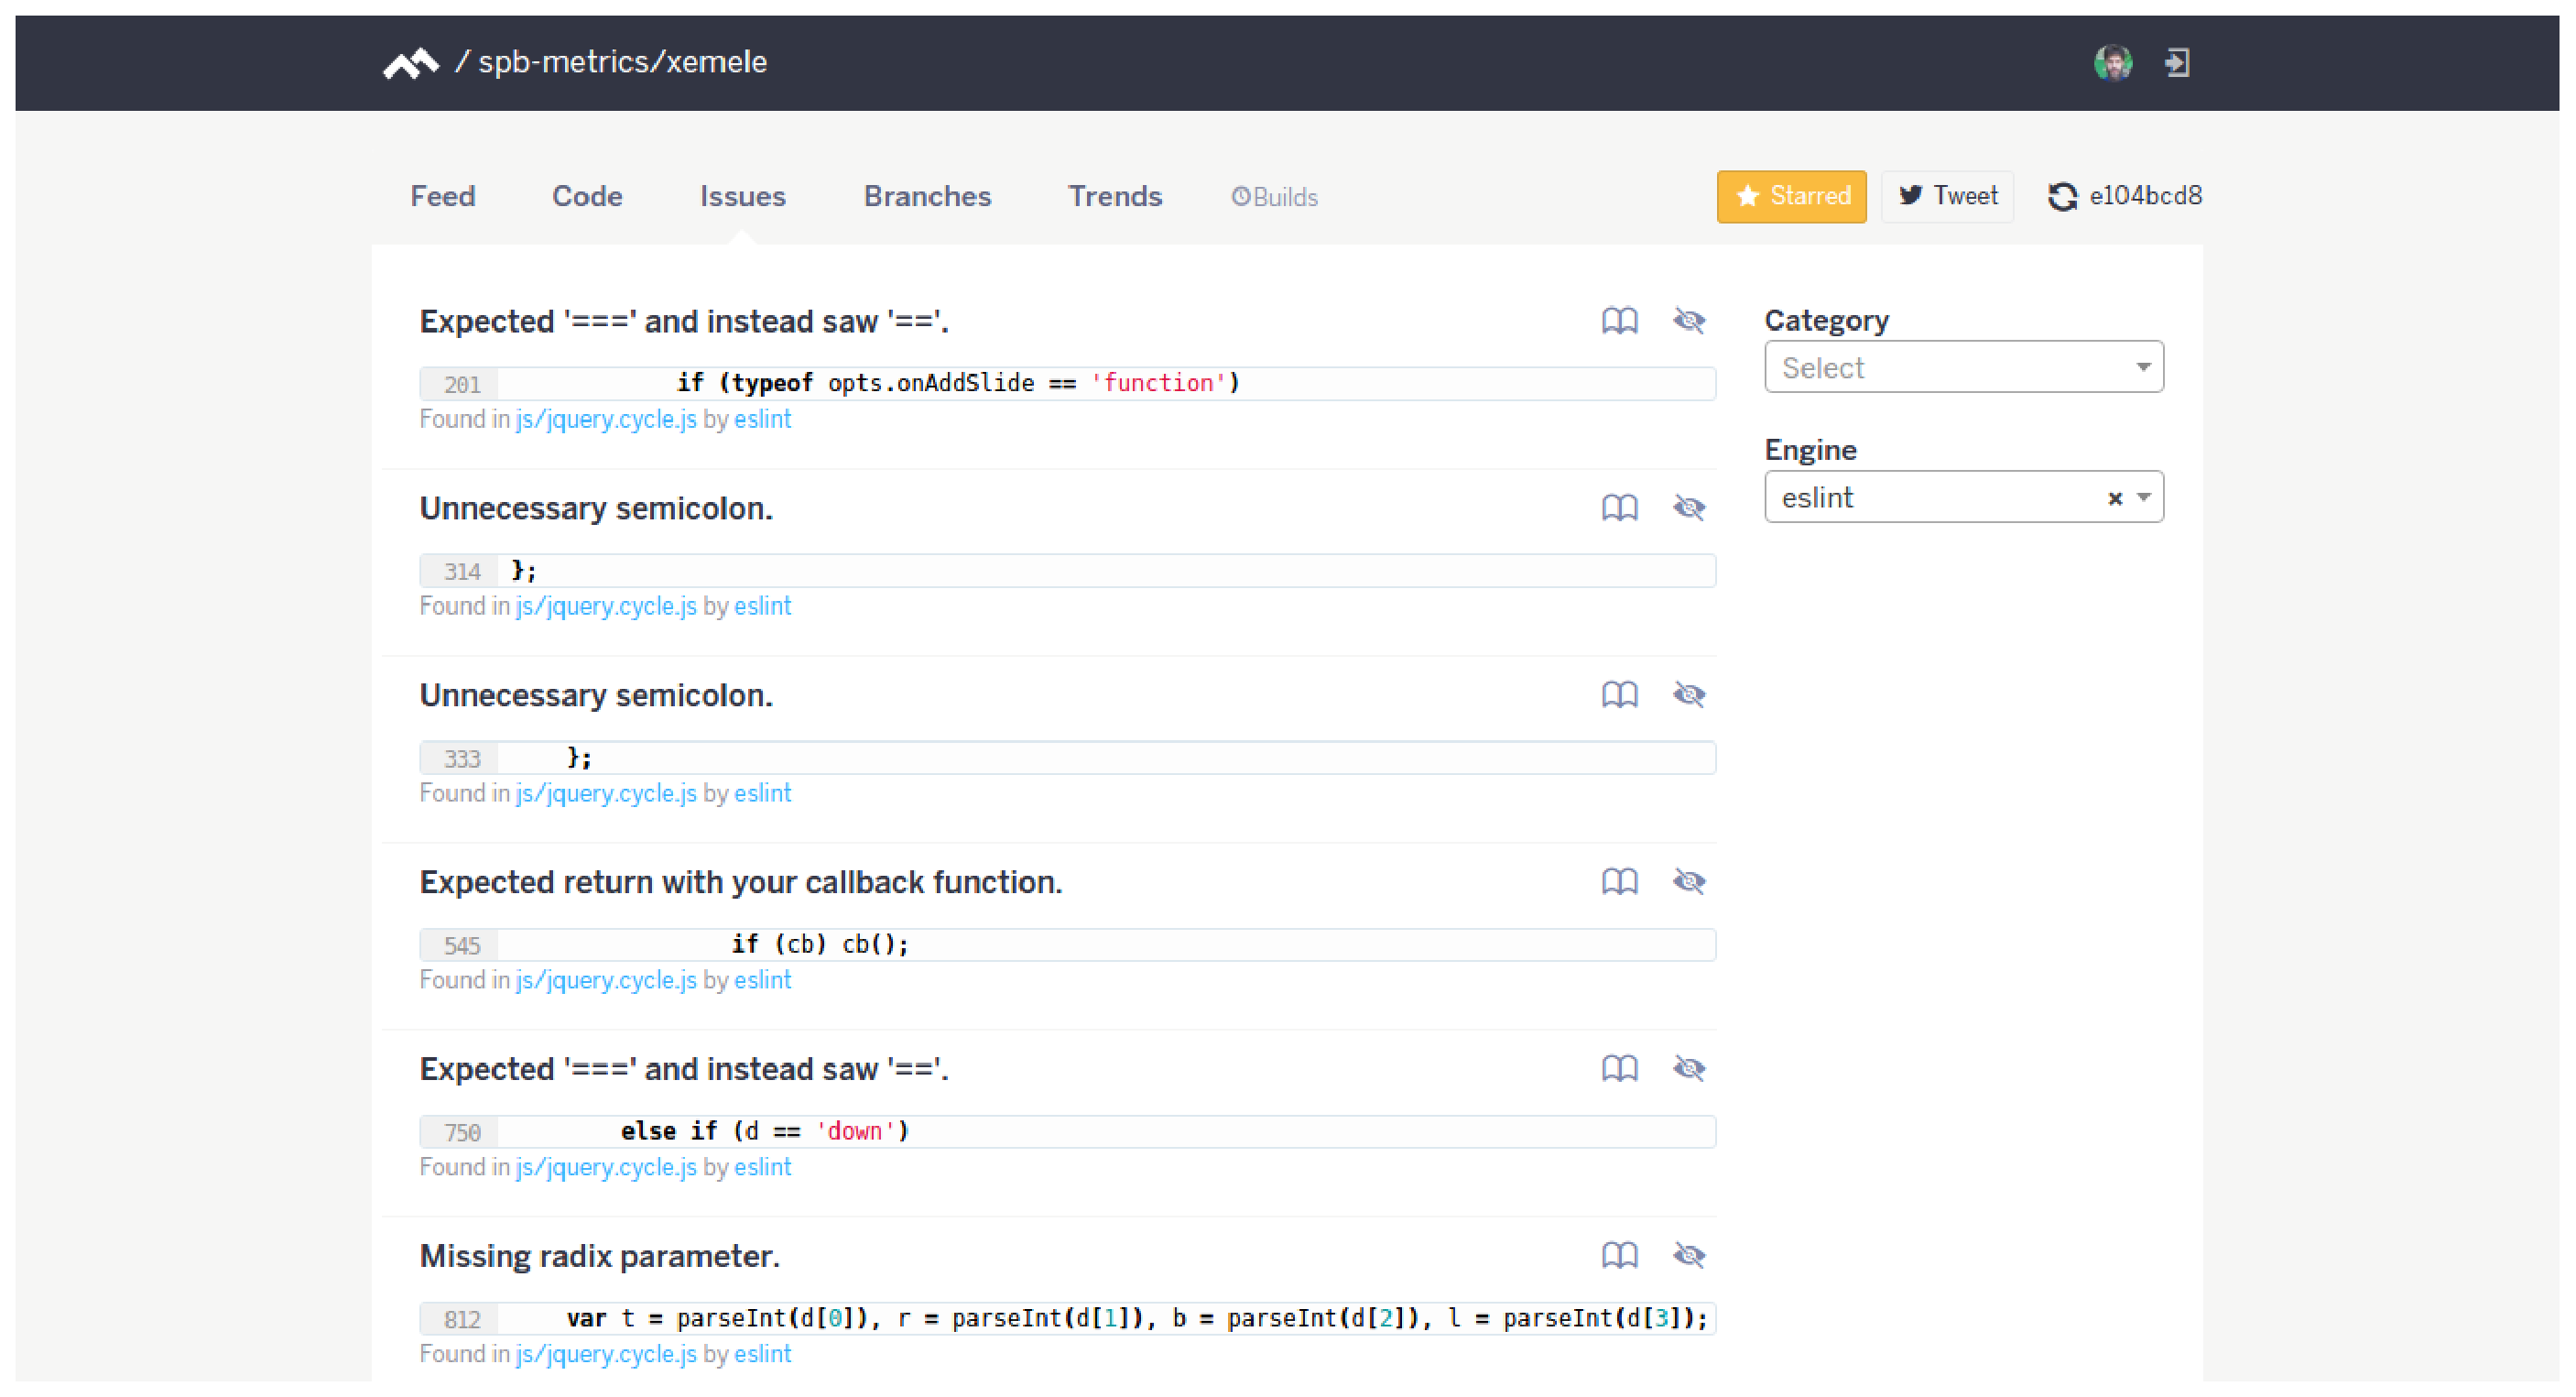
\includegraphics[keepaspectratio=true,scale=0.35]
    {figuras/codeclimate_issues_tab_eslint.eps}
  \caption{Code Climate - Xemelê - Aba \textit{Issues} (ESLint)}
	\label{fig:codeclimate_issues_tab_eslint}
\end{figure}

\newpage

\begin{figure}[!htb]
	\centering
    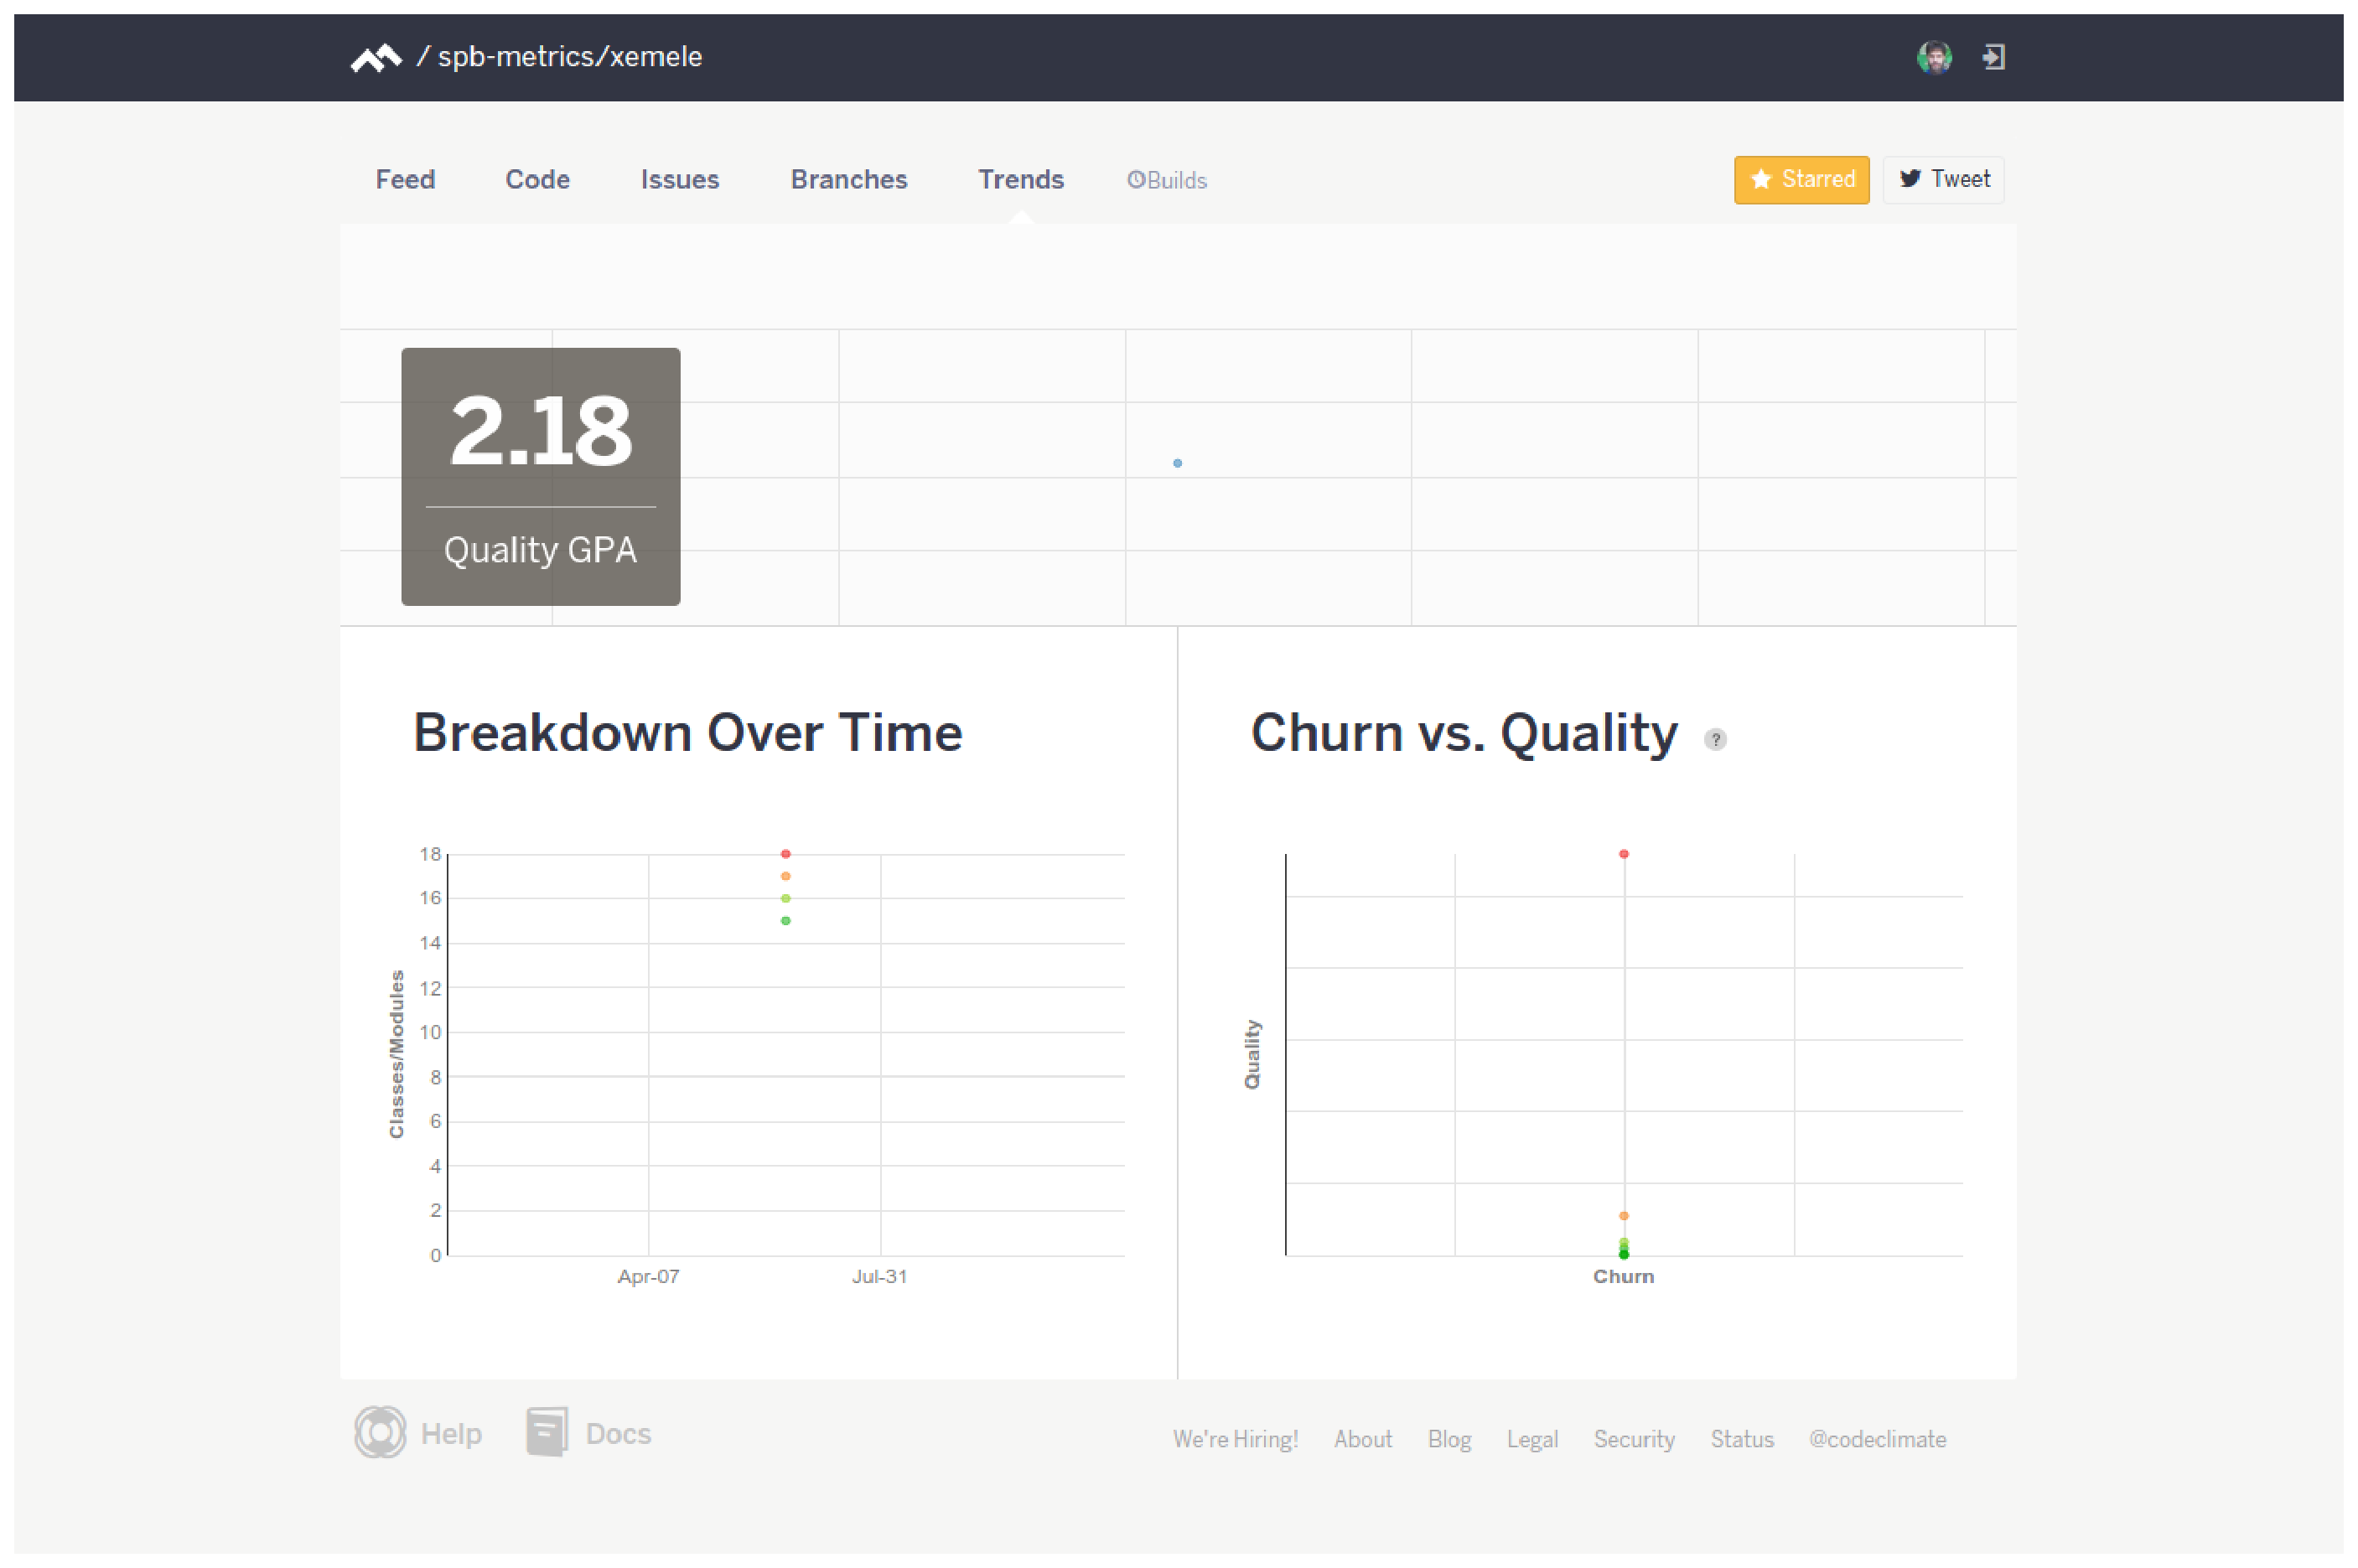
\includegraphics[keepaspectratio=true,scale=0.35]
    {figuras/codeclimate_trends_tab.eps}
  \caption{Code Climate - Xemelê - Aba \textit{Trends}}
	\label{fig:codeclimate_trends_tab}
\end{figure}

\begin{figure}[!htb]
	\centering
    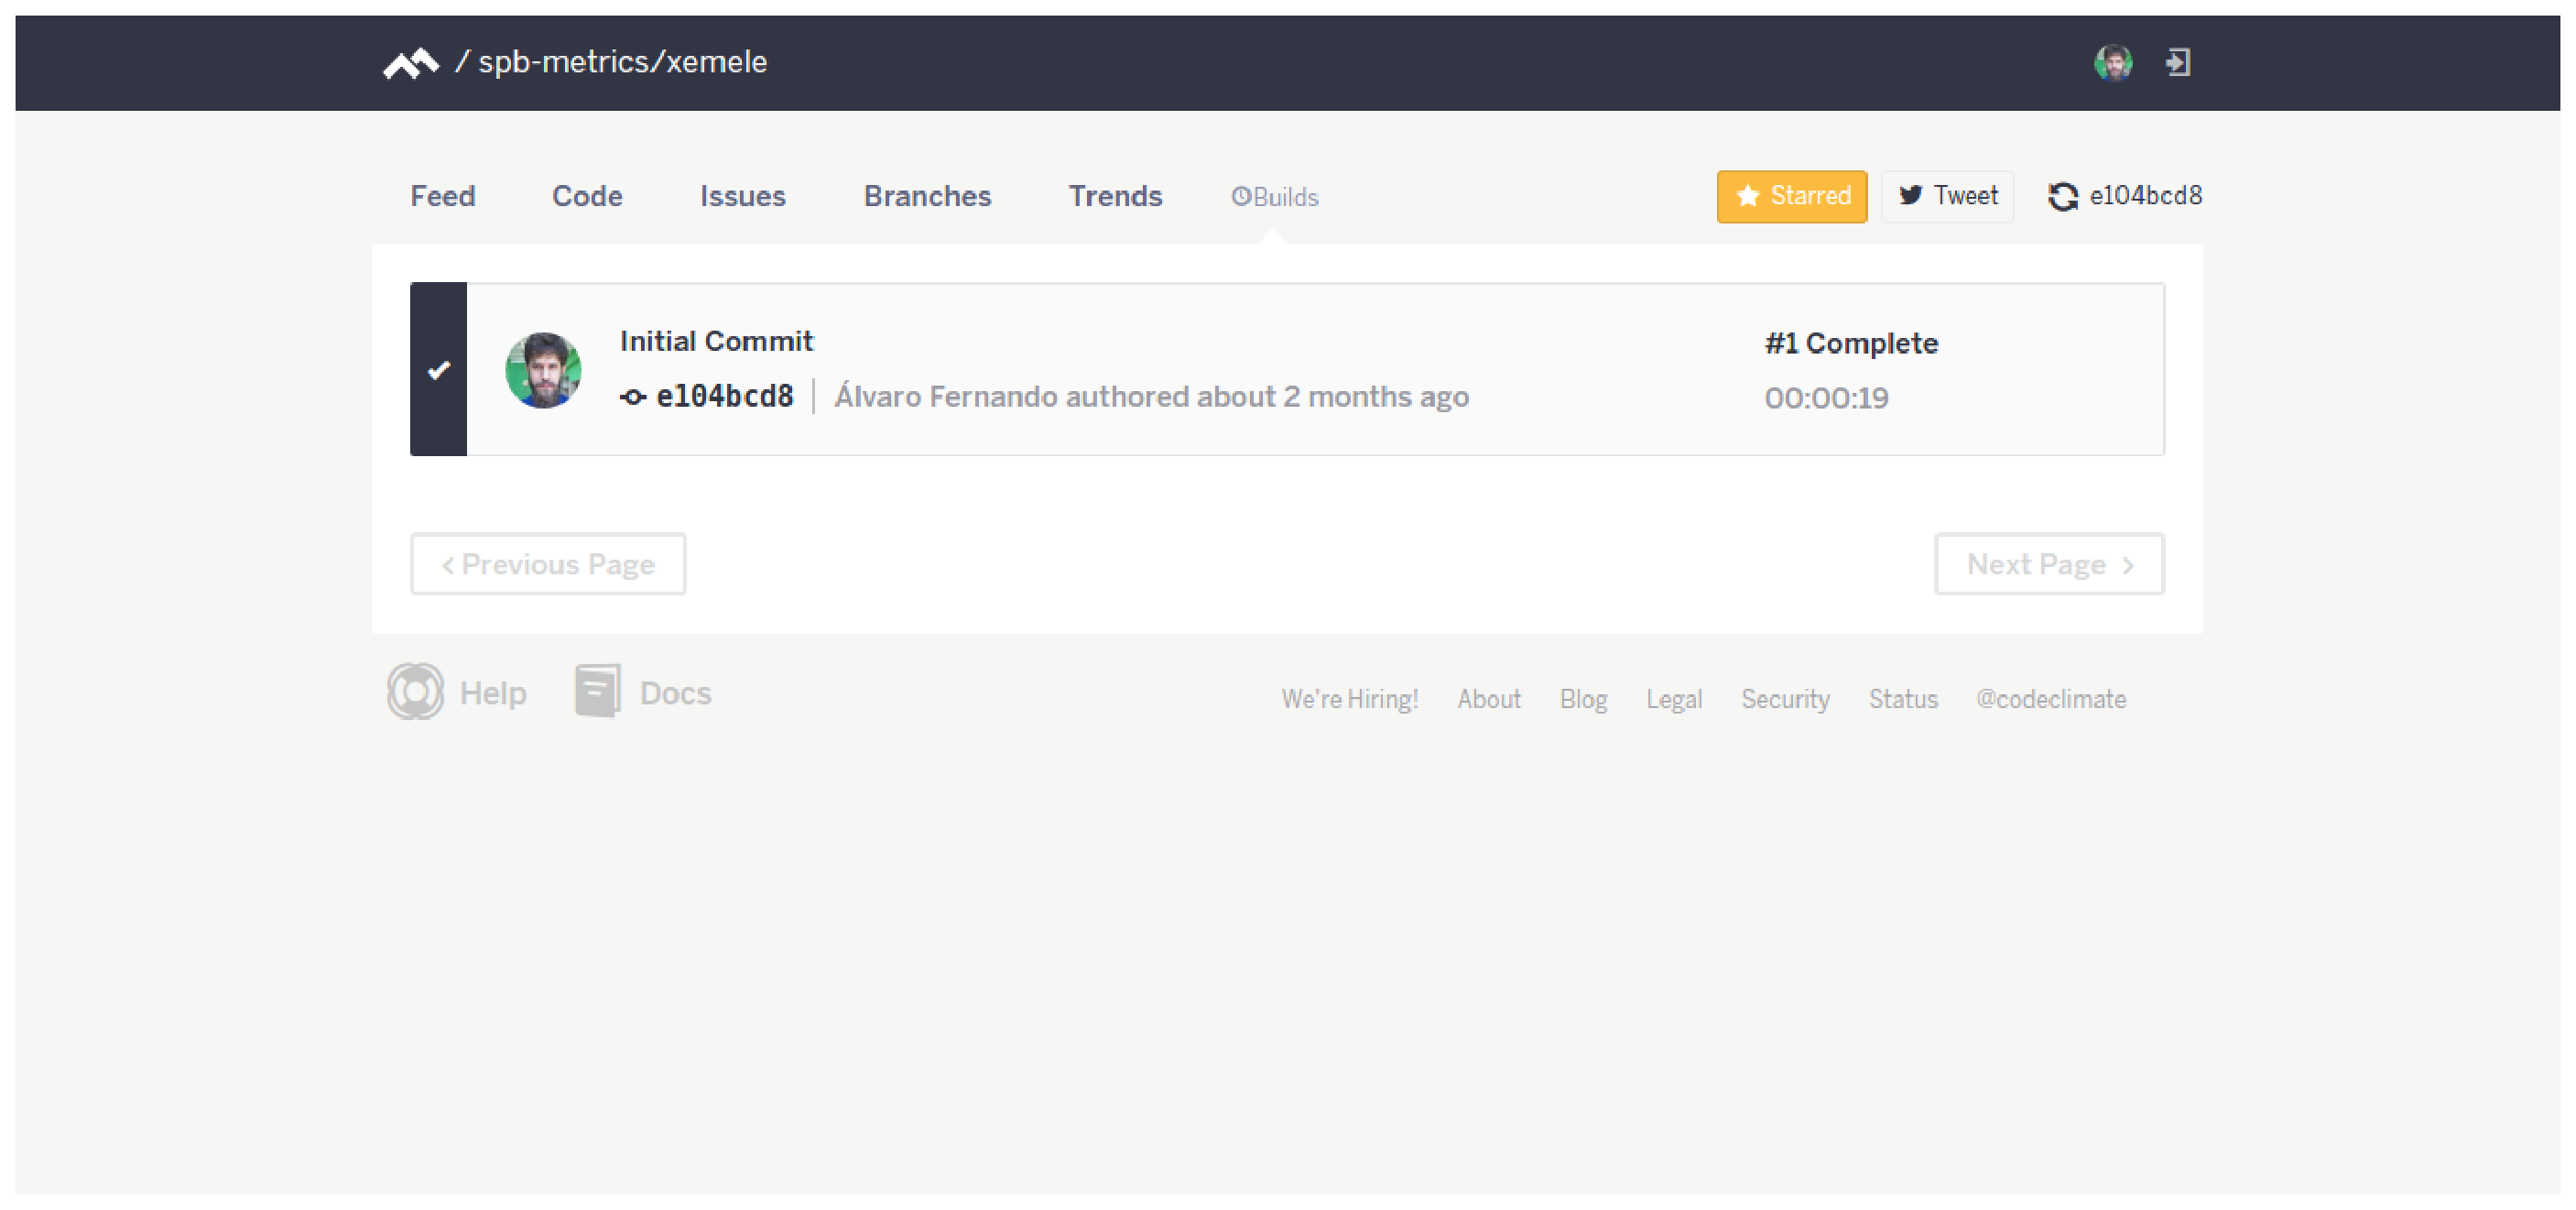
\includegraphics[keepaspectratio=true,scale=0.35]
    {figuras/codeclimate_builds_tab.eps}
  \caption{Code Climate - Xemelê - Aba \textit{Builds}}
	\label{fig:codeclimate_builds_tab}
\end{figure}

As imagens acima, mostram parte dos resultados obtidos na análise do Xemelê no
Code Climate. A quantidade de informação é significativamente maior que no Mezuro.
Isso é devido ao fato de que, no Code Climate, análises do CSS, código duplicado
e de código Javascript foram feitas. Porém, considerando as análises de código
Javascript, o resultado exposto é referente à análise de bibliotecas de
terceiros (jQuery) e não necessariamente do projeto Xemelê.

\section{Melhorias de Back-End no Mezuro}

Mesmo não sendo o objetivo deste trabalho, a análise exploratória levou à
indicação de algumas melhorias de Back-End. Não era esperado encontrar certos
problemas com as avaliações dos projetos, porém, alguns deles
são: falta de espaço em disco para o download dos projetos, falha no
redirecionamento após a adição do projeto, queda dos serviços no servidor de
produção, lentidão e falhas de processamento. A equipe do Mezuro
esteve sempre a disposição para auxiliar na explanação e resolução destas
falhas, seja via canal no IRC, via e-mail ou via \textit{issues} no Github do
projeto. Estes impedimentos foram de fato detectados pela equipe na análise dos
\textit{logs} e nos relatos feitos. Foi catalogado os seguintes problemas:

\begin{itemize}
  \item \textbf{Capacidade de Disco}:
    \begin{itemize}

      \item Handle full disk (Lidar com o disco cheio)
      \footnote{\url{https://github.com/mezuro/kalibro\_processor/issues/203}}:
        suspeita-se que quando o disco está cheio, o processamento para, levando
        o processo de análise para o estado de finalizado/pronto, mas não
        informando ao usuário tal problema e/ou o estado.

        A sugestão para tratar desse erro é verificar a capacidade do
        disco antes do download e/ou notificar sobre os erros ocorridos.

      \item Schedule removal job for repositories with no periodicity (Tarefa
      agendada de remoção de repositórios sem frequência de reprocessamento)
      \footnote{\url{https://github.com/mezuro/kalibro\_processor/issues/204}}:
        é considerado desnecessário manter um repositório em que não foi
        configurado uma frequência de reprocessamento. Esta solução pode sanar
        os problemas de capacidade de disco.

      \item Store SCM reference on a given processing (Armazenar a referência ao
      sistema de controle de versão de um projeto em um determinado
      processamento)
      \footnote{\url{https://github.com/mezuro/kalibro\_processor/issues/205}}:
        solução esta que pode auxiliar na correlação entre o repositório/código
        apagado do disco com os resultados no futuro.

      \item Is the aggregation working correctly? (A agregação está funcionando
      corretamente?)
      \footnote{\url{https://github.com/mezuro/kalibro\_processor/issues/206}}:
        Algumas notas dadas aos projetos avaliados estão retornando um valor
        diferente do esperado, julgando pelas notas dos submódulos.

    \end{itemize}
  \item \textbf{Lentidão de Processamento}:
    \begin{itemize}

      \item Slow processings (Processamentos Lentos)
      \footnote{\url{https://github.com/mezuro/kalibro\_processor/issues/207}}:
        Alguns processamentos estão levando certa de 30 minutos para
        finalizarem. Foi sugerido, portanto, alguns testes de performance,
        investigações de possíveis causas e melhoria de determinadas etapas do
        processamento;

      \item Multiple calls to process trigger multiple redundant periodic
      processings (Chamadas excessivas para o gatilho de processo com muitos
      períodos de processamento redundante)
      \footnote{\url{https://github.com/mezuro/kalibro\_processor/issues/208}}:
        muitas chamadas para os métodos de processamento estão sendo feitas, o
        que gera muitos processos e muito desperdício de tempo.

        Uma solução é a separação de diferentes filas de requisições para
        diferentes eventos.

      \item Separate processings in multiple queues (Processos separados por
      várias filas)
      \footnote{\url{https://github.com/mezuro/kalibro\_processor/issues/209}}:
        A sugestão é a separação de três filas de requisição de processamento,
        com prioridades distintas. Maior para novos repositórios avaliados,
        baixa prioridade para os reprocessamentos e o isolamento dos
        processamentos periódicos

    \end{itemize}
  \item \textbf{Falhas de Processamento}:
    \begin{itemize}
      \item Handle `Metric configuration has already been taken` error (Lidar
      com o erro ``Configuração de Métrica já foi selecionada'')
      \footnote{\url{https://github.com/mezuro/kalibro\_processor/issues/210}};

      \item Failed processing (Falha no Processamento)
      \footnote{\url{https://github.com/mezuro/kolekti\_radon/issues/3}}:
        um erro não determinado tem feito o processamento da avaliação falhar.
        A investigação e prevenção deste erro pode ser uma solução;

      \item Docker runner timeout (Agente de execução do Docker está retornando
      erro de tempo esgotado
      \footnote{\url{https://github.com/mezuro/kolekti\_cc\_phpmd/issues/11}}:
        um processo está esgotando o tempo de execução e sendo finalizado.
    \end{itemize}
\end{itemize}
